\documentclass[12pt]{beamer}
\usetheme{Madrid}
\usepackage[utf8]{inputenc}
\usepackage{amsmath}
\usepackage{amsfonts}
\usepackage{amssymb}
\usepackage{graphicx}
\usepackage{caption}
\usepackage{subcaption}
\usepackage{movie15}
\setcounter{tocdepth}{4}
\setcounter{secnumdepth}{4}
\usepackage{listings}
\title{Convolutional Neural Networks}
%\setbeamercovered{transparent} 
%\setbeamertemplate{navigation symbols}{} 
%\logo{} 
%\institute{} 
%\date{} 
%\subject{} 

\author{
\linebreak
Julius Taylor \\ \texttt{5210444} \\ \href{mailto:s8423760@stud.uni-frankfurt.de}{s8423760@stud.uni-frankfurt.de}
 \and   
 \linebreak
Shawn Cala \\ \texttt{4921431} \\ \href{mailto:shawn.cala@gmail.com}{shawn.cala@gmail.com}
}

\begin{document}

\begin{frame}
\titlepage
\end{frame}
\frame{\frametitle{Table of Contents}\tableofcontents} 
\section{Background}
\subsection{Neural Networks}
\begin{frame}{Neural Networks}

Primary motivation: Neural Networks mathematically simulate biological functionalities of the human brain
\begin{figure}
\begin{subfigure}{.5\textwidth}
  \centering
  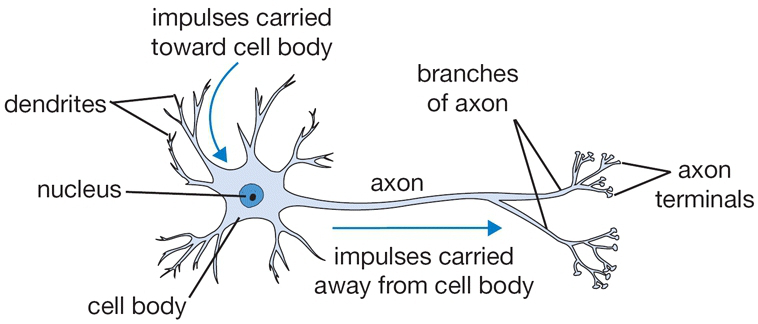
\includegraphics[width=\linewidth,height=0.35\textheight]{images/neuron.png}
  \caption{biological model}
  \label{fig:sub1}
\end{subfigure}%
\begin{subfigure}{.5\textwidth}
  \centering
  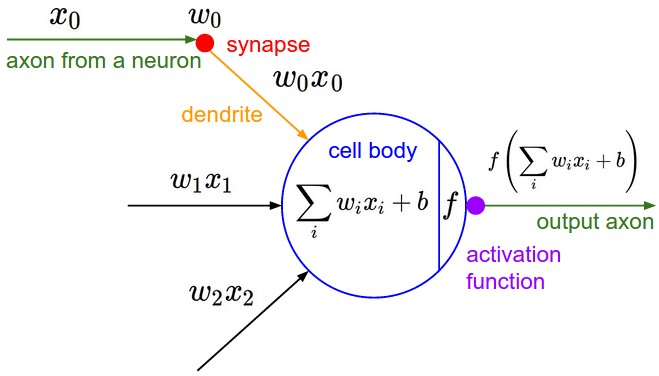
\includegraphics[width=\linewidth,height=0.35\textheight]{images/neuron_model.jpeg}
  \caption{mathematical representation}
  \label{fig:sub2}
\end{subfigure}
\caption{neuronal model and computational abstraction}
\label{fig:abstract}
\end{figure}

\end{frame}
\subsection{Structure}
\begin{frame}{Structure}
Neural Networks generally contain:
  \begin{itemize}
     \item an n-dimensional input 
     \item one or many layers of interconnected neurons
     \item an output-layer
  \end{itemize}
\begin{figure}
\centering
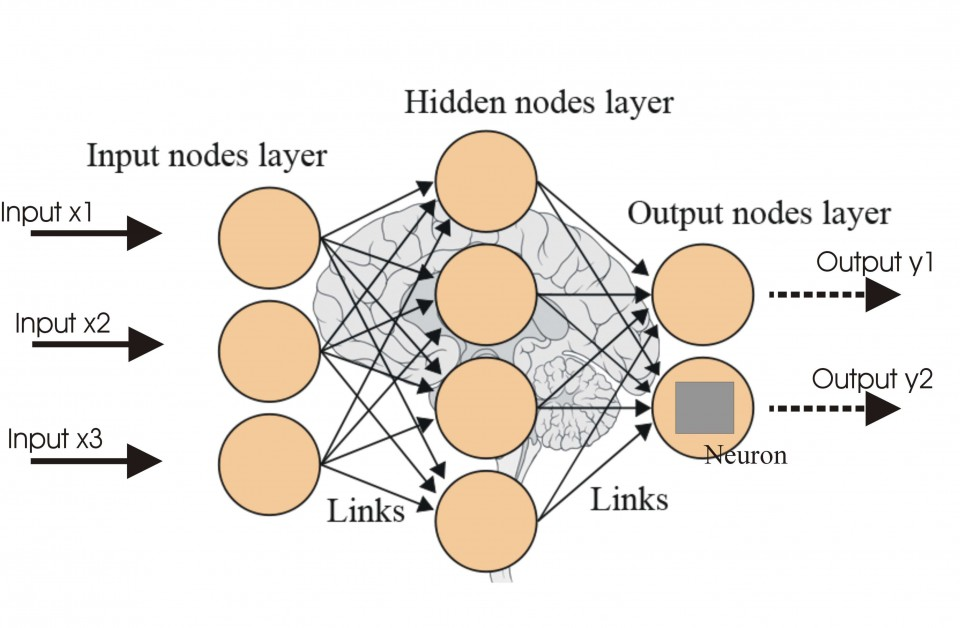
\includegraphics[width=0.5\linewidth]{images/principle.jpg}
\caption{Basic concept of a Neural Network}
\label{fig:principle}

\end{figure}

\end{frame}

\begin{frame}{The Problem Space}
  \begin{itemize}
  \item image classification: Image $\rightarrow$ class that best describes the image (eg. 'Cat', 'Ship')
  \item recognizing patterns and generalizing from prior knowledge 
  \item figure out features, that describe things
  \end{itemize}
\end{frame}

\section{Convolutional Neural Networks}
\subsection{Problem Space}






\begin{frame}{Problems with image classification}
  \begin{itemize}
     \item naive approach: comparing pixels one by one
     \item very sensitive to small changes and does not generalize	
  \end{itemize}
\begin{figure}
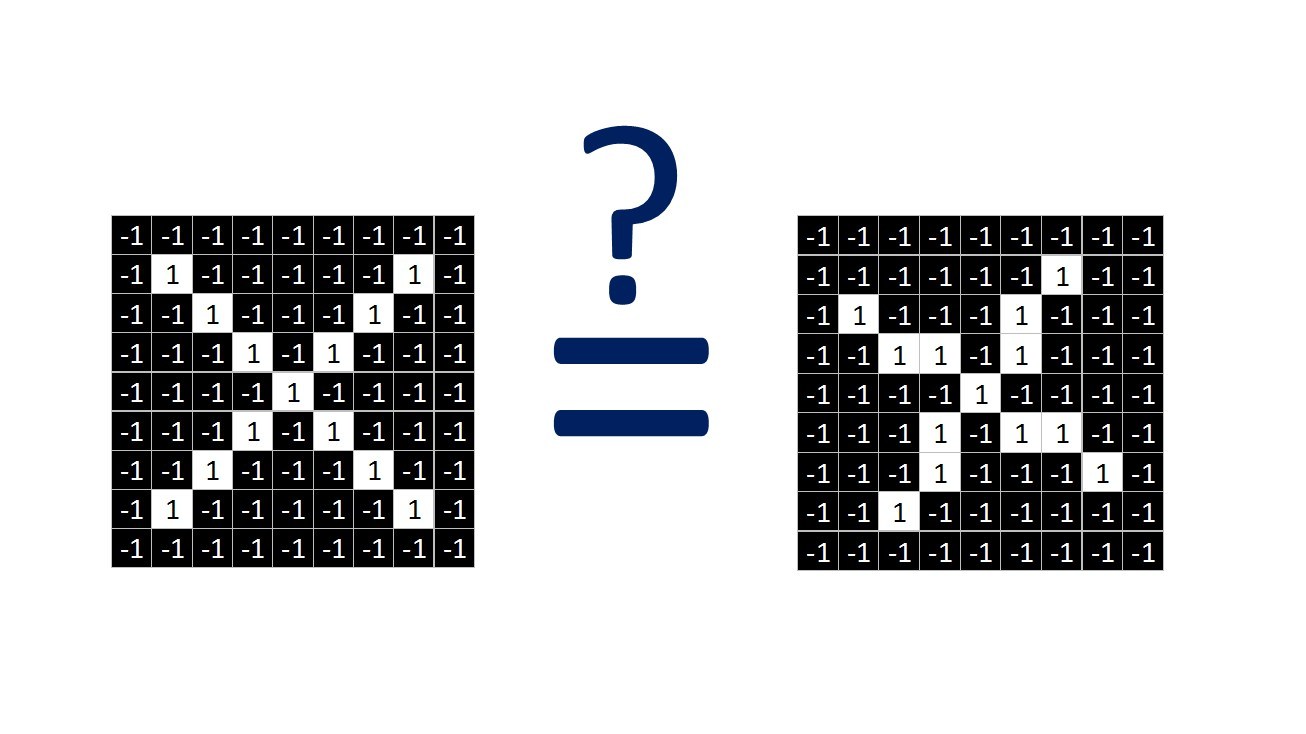
\includegraphics[width = 0.4\linewidth]{images/equal.jpg}
\label{fig:principle}
\end{figure}
\end{frame}
\begin{frame}{Problems with image classification}
\begin{figure}
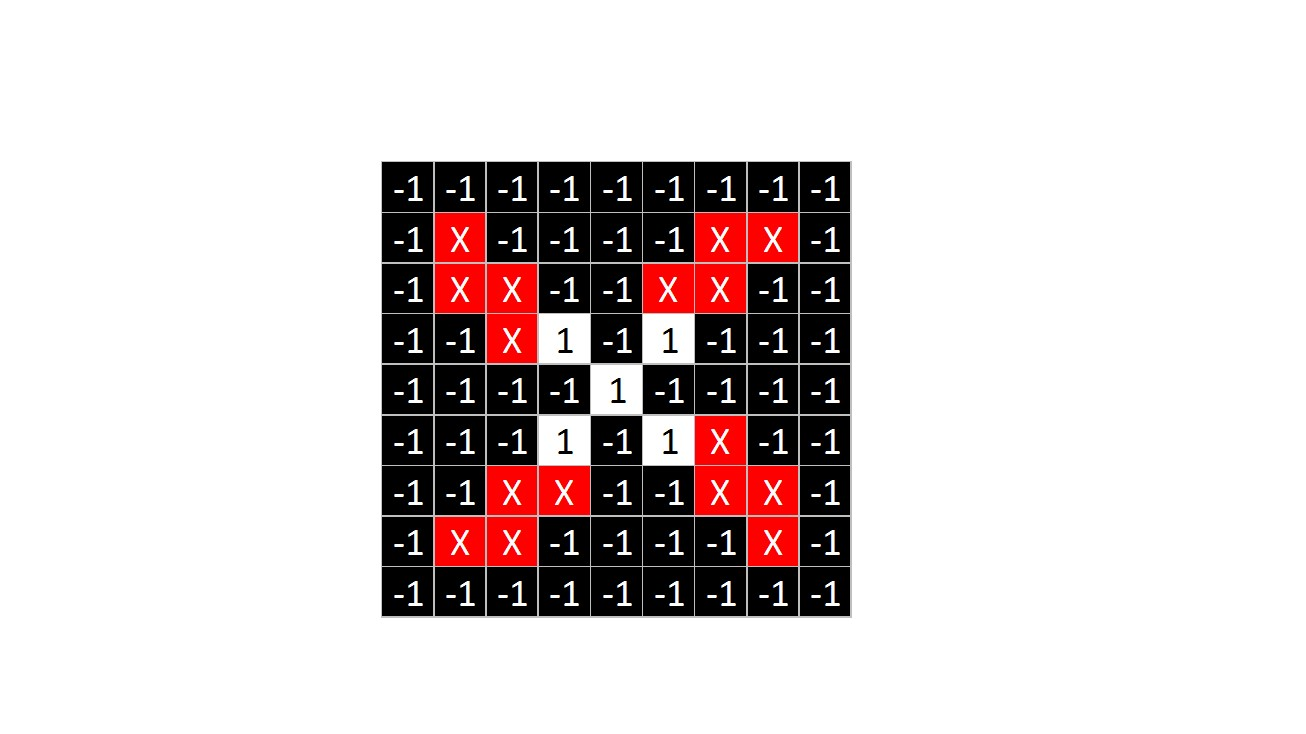
\includegraphics[width = 0.8\linewidth]{images/neq.jpg}
\caption{Visualizing what computers see}
\label{fig:principle}
\end{figure}
\end{frame}
\begin{frame}{Problems with image classification}
\begin{figure}
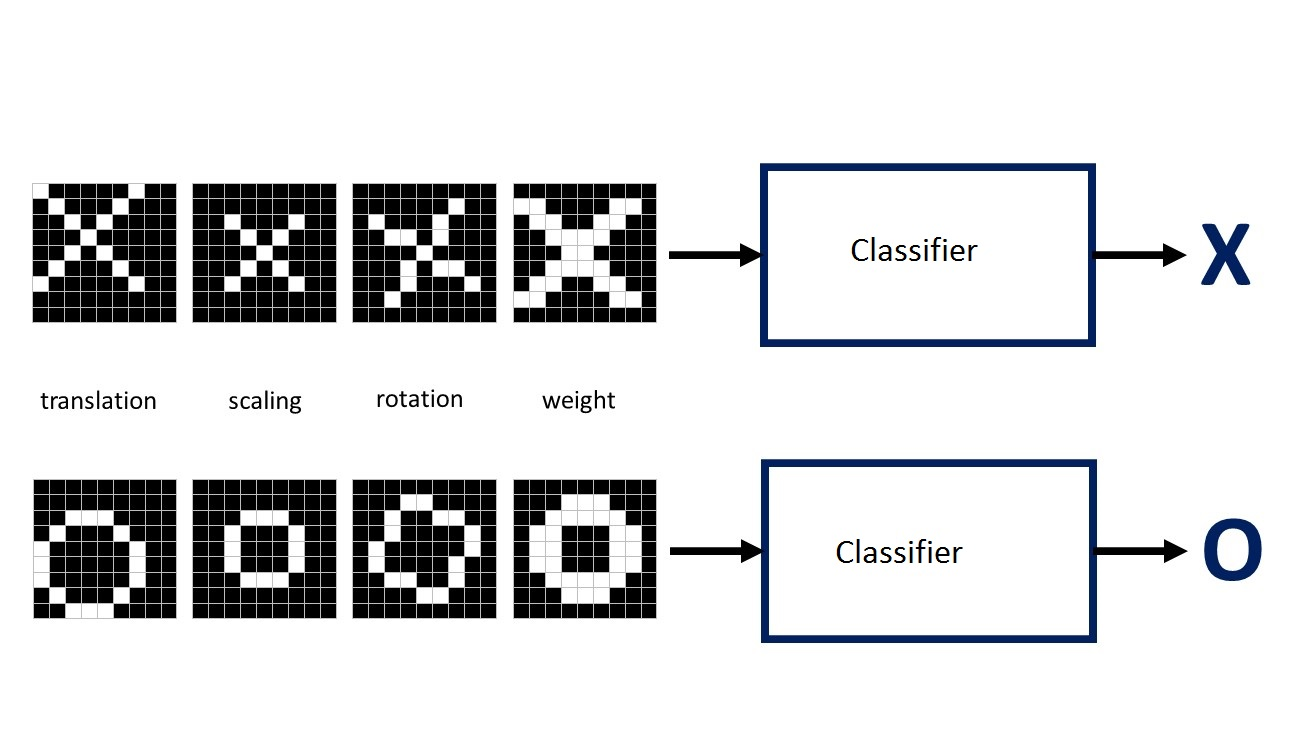
\includegraphics[width = 0.8\linewidth]{images/diff.jpg}
\label{fig:principle}
\end{figure}
\end{frame}



\begin{frame}{What makes us conclude that two pictures match?}
\begin{figure}
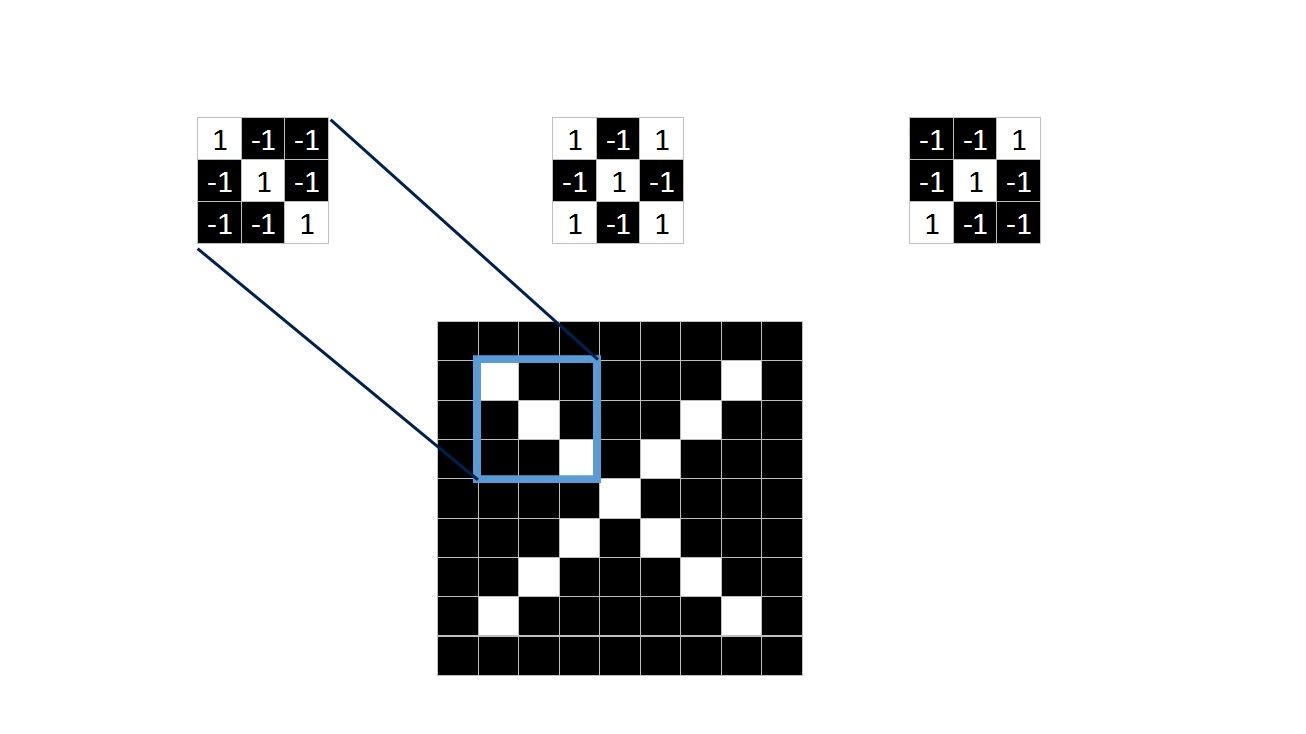
\includegraphics[width = 0.8\linewidth]{images/feat1.jpg}
\label{fig:principle}
\end{figure}
\end{frame}

\begin{frame}{What makes us conclude that two pictures match?}
\begin{figure}
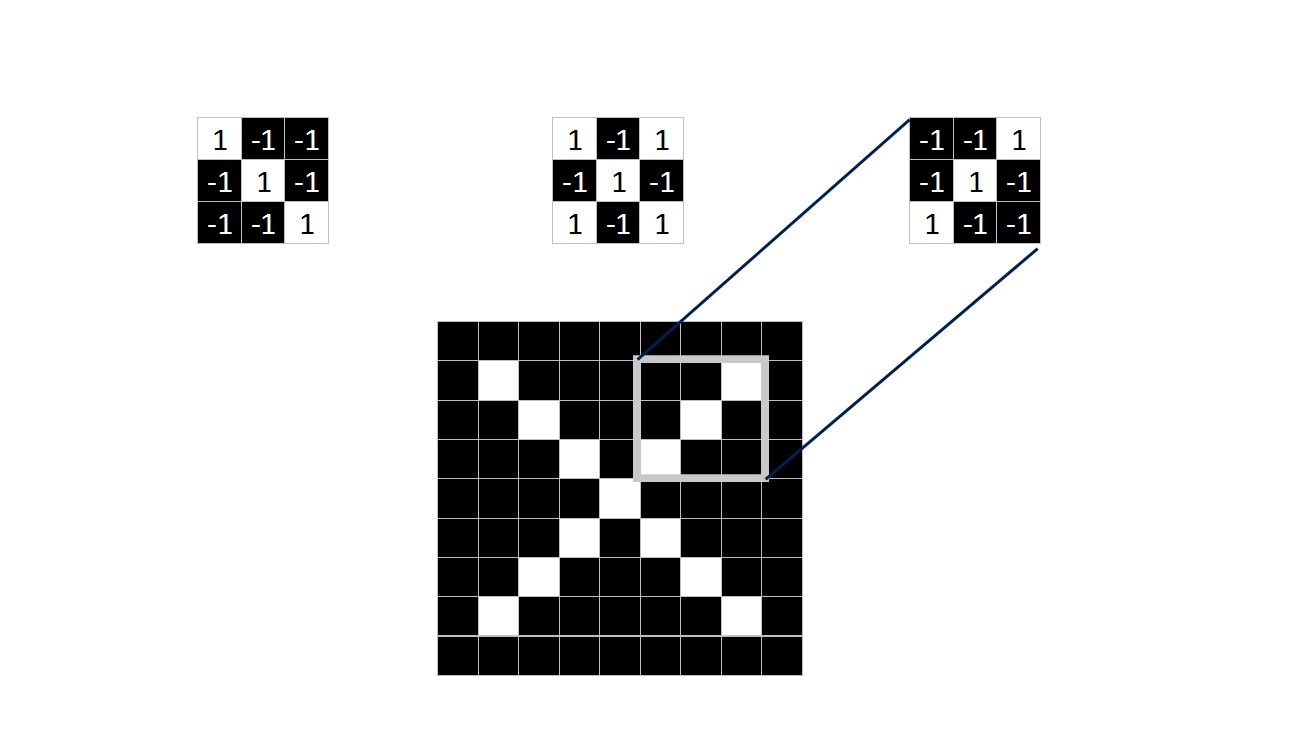
\includegraphics[width = 0.8\linewidth]{images/feat2.jpg}
\label{fig:principle}
\end{figure}
\end{frame}

\begin{frame}{What makes us conclude that two pictures match?}
\begin{figure}
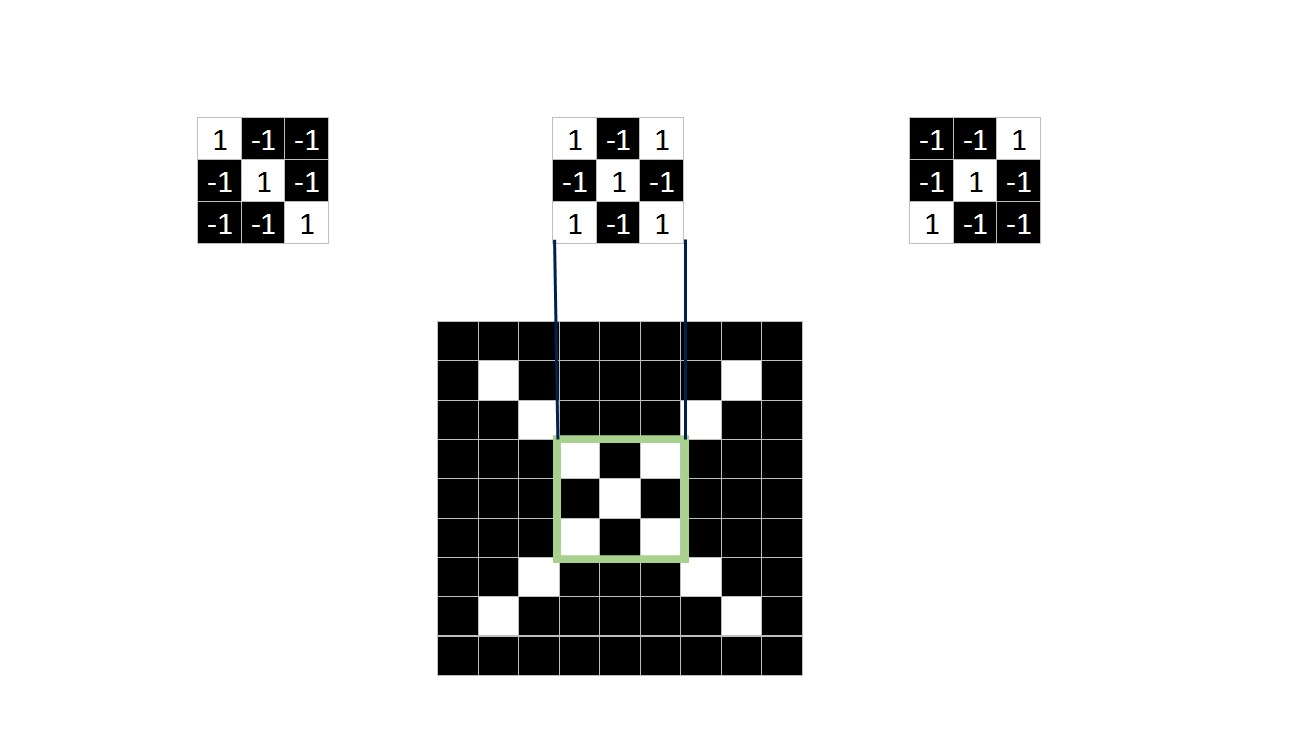
\includegraphics[width = 0.8\linewidth]{images/feat3.jpg}
\label{fig:principle}
\end{figure}
\end{frame}

\begin{frame}{What makes us conclude that two pictures match?}
\begin{figure}
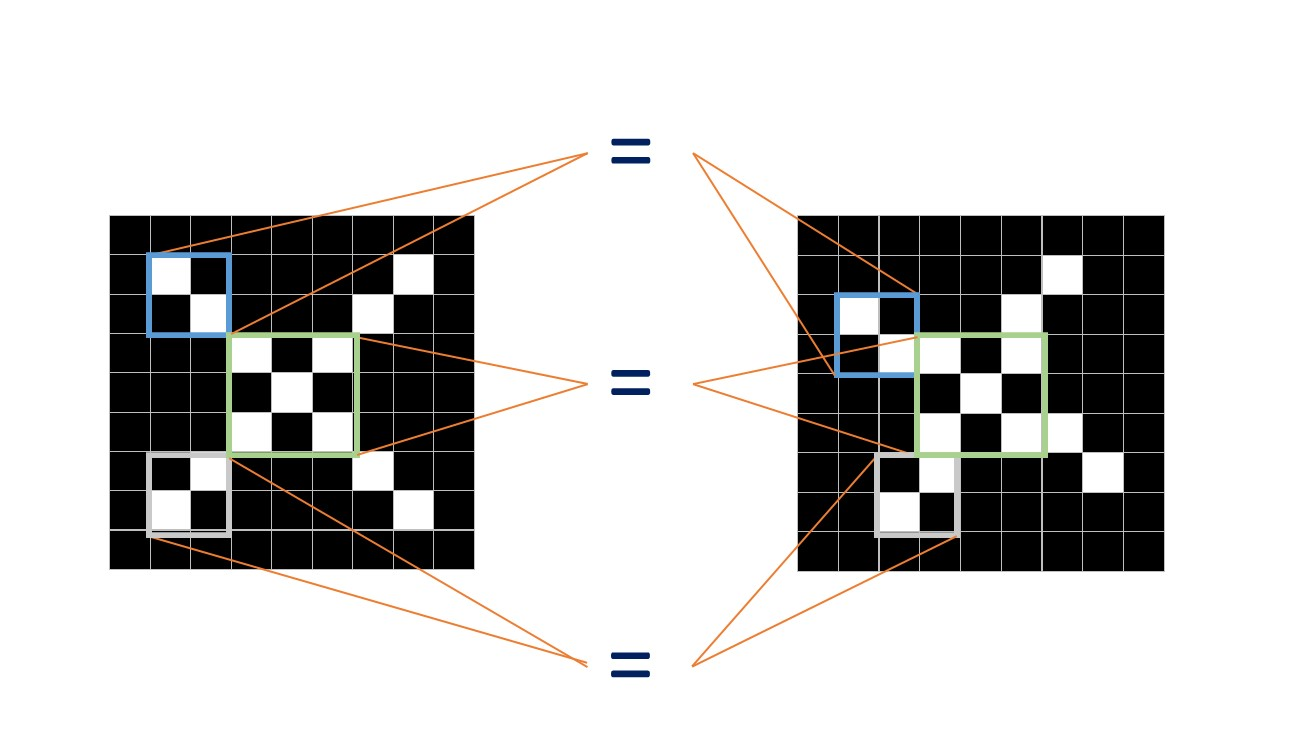
\includegraphics[width = 0.8\linewidth]{images/features.jpg}
\label{fig:principle}
\end{figure}
\end{frame}



\begin{frame}{Solution: CNN's}
Convolutional Neural Networks (CNNs) are a subtype of Neural Networks:
  \begin{itemize}
  	\item is a type of feed-forward network
  	\item structure inspired by the animal visual cortex
     \item uses many identical copies of the same neuron
     \item express computationally extensive models while keeping weights to learn small
     \item breakthrough results in pattern recognition problems
     
  \end{itemize}
\end{frame}

\subsection{Concept}

\begin{frame}{Structure}
\begin{figure}
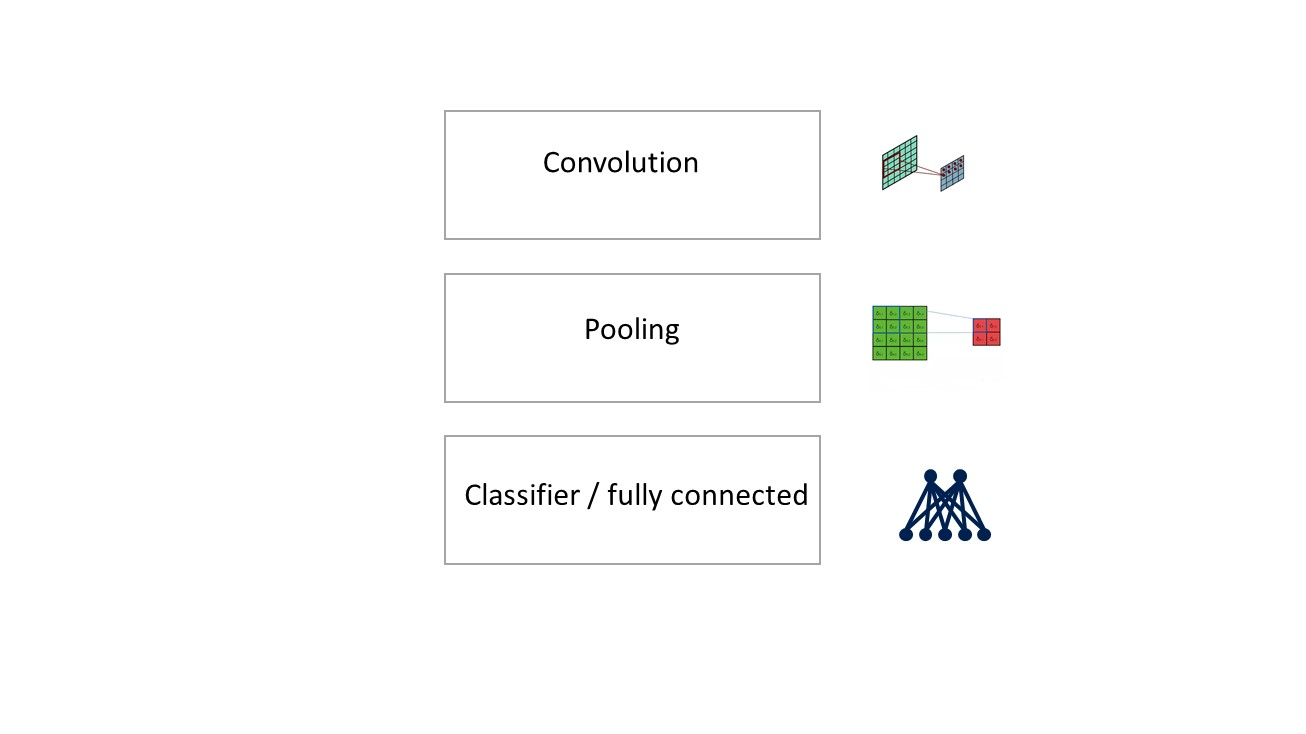
\includegraphics[width = 1\linewidth]{images/struct.jpg}
\label{fig:principle}
\end{figure}
\end{frame}

\begin{frame}{Structure}
\begin{figure}
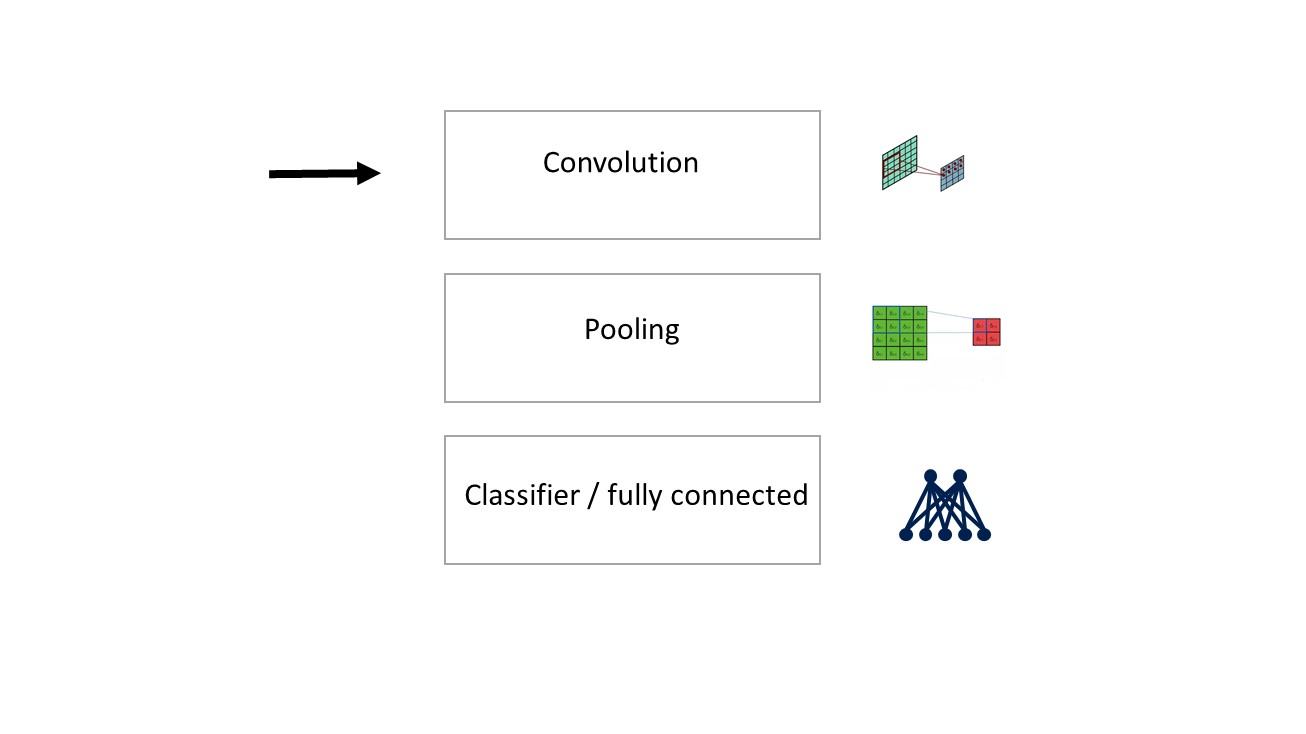
\includegraphics[width = 1\linewidth]{images/struct1.jpg}
\label{fig:principle}
\end{figure}
\end{frame}

\begin{frame}{Finding Features}
  \begin{itemize}
  \item We find features in a picture by filtering

  \end{itemize}
\begin{figure}
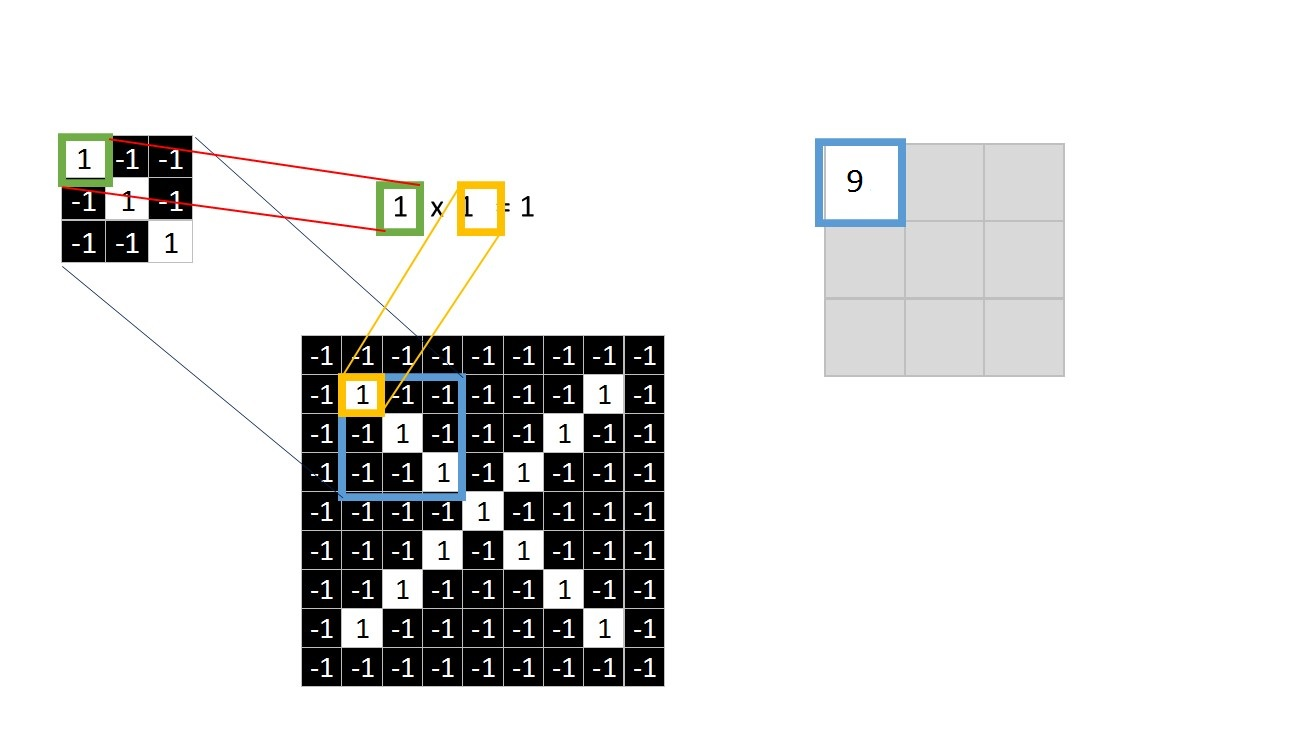
\includegraphics[width = 0.8\linewidth]{images/convolution.jpg}
\label{fig:principle}
\end{figure}
\end{frame}

\begin{frame}{Finding Features}
\begin{figure}
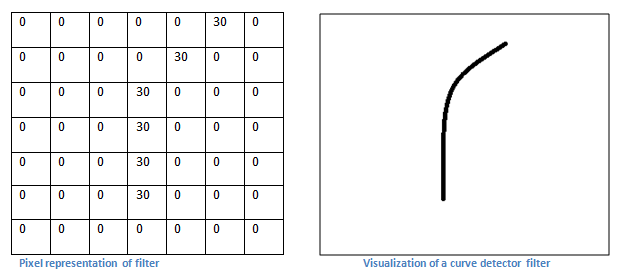
\includegraphics[width = 0.8\linewidth]{images/Filter.png}
\label{fig:principle}
\end{figure}
\end{frame}

\begin{frame}{Finding Features}
\begin{figure}
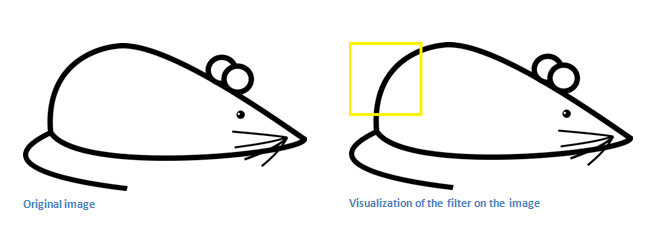
\includegraphics[width = 0.8\linewidth]{images/mouse.png}
\label{fig:principle}
\end{figure}
\end{frame}

\begin{frame}{Finding Features}
\begin{figure}
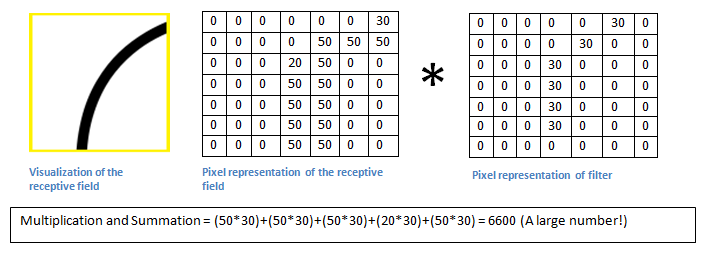
\includegraphics[width = 0.8\linewidth]{images/mousehi.png}
\label{fig:principle}
\end{figure}
\end{frame}

\begin{frame}{Finding Features}
\begin{figure}
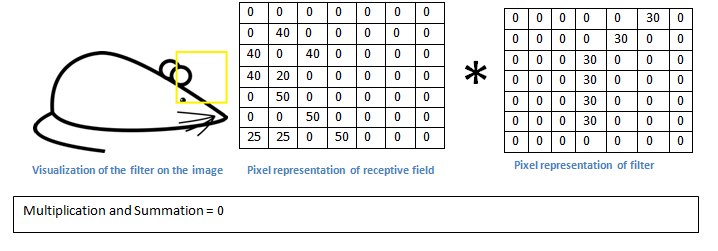
\includegraphics[width = 0.8\linewidth]{images/mouselo.png}
\label{fig:principle}
\end{figure}

\end{frame}

\subsection{Kernel function}


\begin{frame}{Finding Features}
\begin{figure}
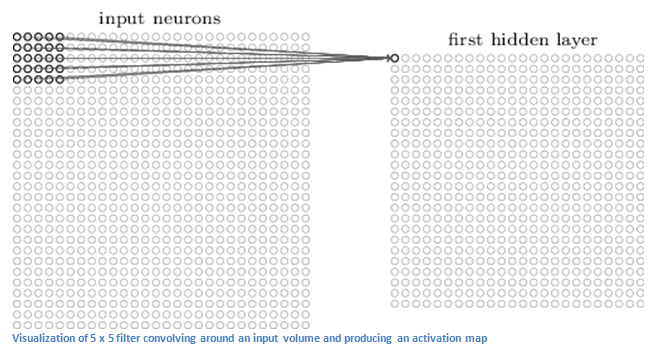
\includegraphics[width = 0.6\linewidth]{images/activation.png}
\label{fig:principle}
\end{figure}
$(f\ast g)(c_1, c_2) = \sum_{a_1, a_2} f(a_1, a_2) \cdot g(c_1-a_1,~ c_2-a_2)$

\end{frame}

\begin{frame}{First Trick: Convolutions}
\begin{figure}
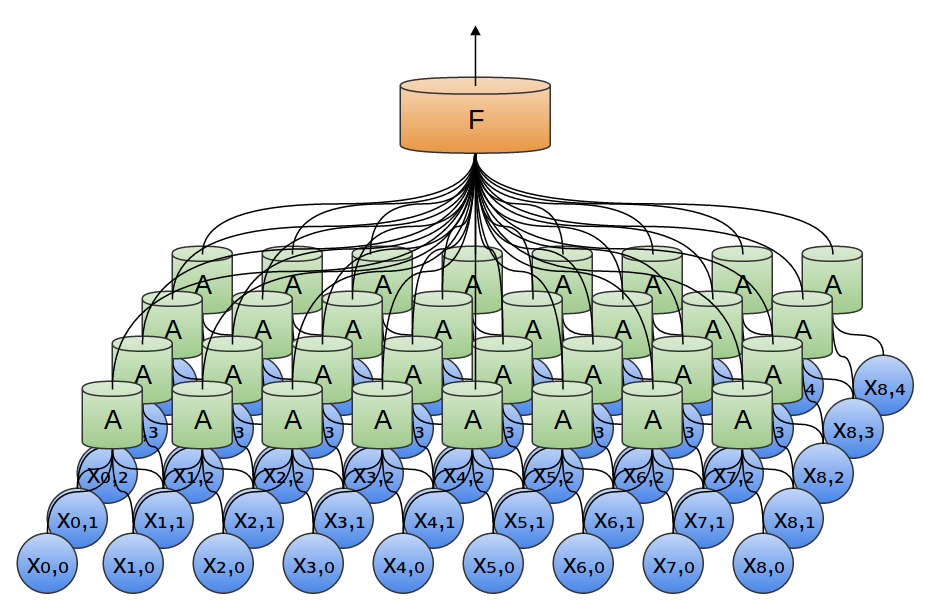
\includegraphics[width = 0.8\linewidth]{images/convnet.png}
\caption{A convolutional layer fed into a fully connected layer}
\label{fig:principle}
\end{figure}
\end{frame}

\begin{frame}{Structure}
\begin{figure}
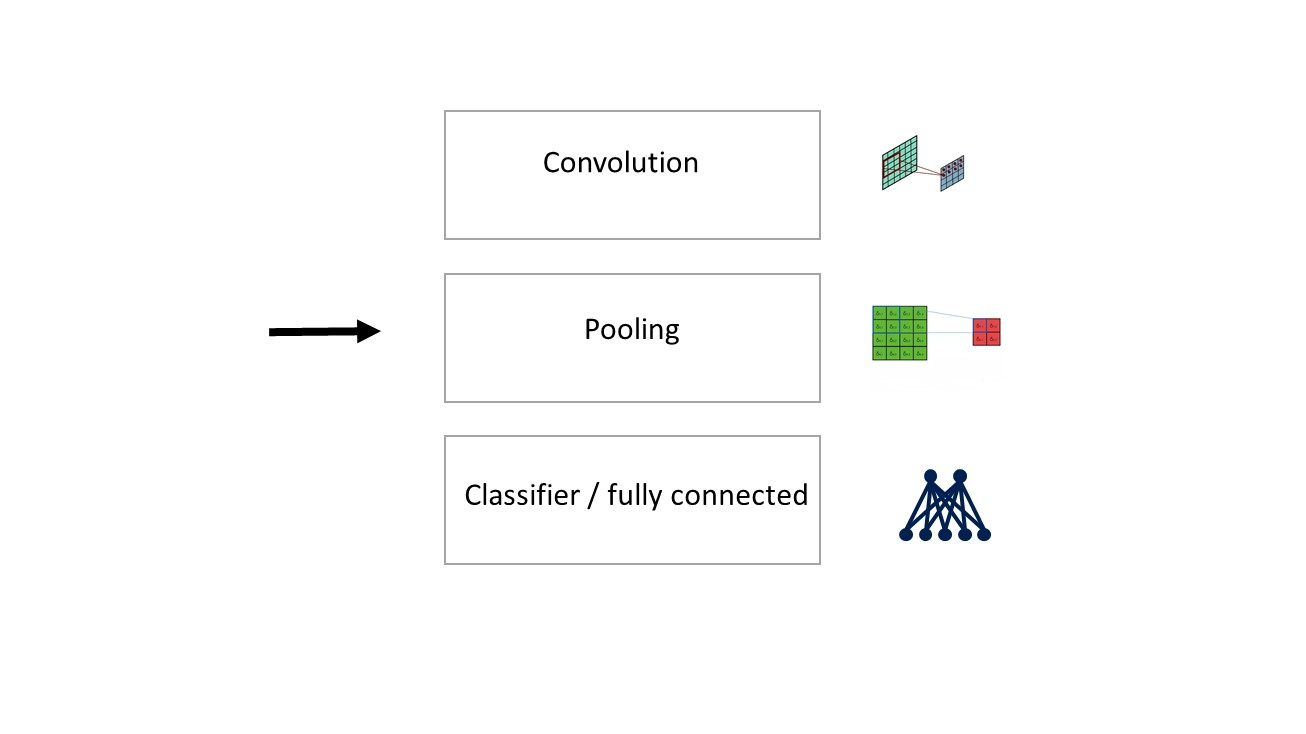
\includegraphics[width = 1\linewidth]{images/struct2.jpg}
\label{fig:principle}
\end{figure}
\end{frame}

\begin{frame}{Second Trick: Pooling}
\begin{figure}
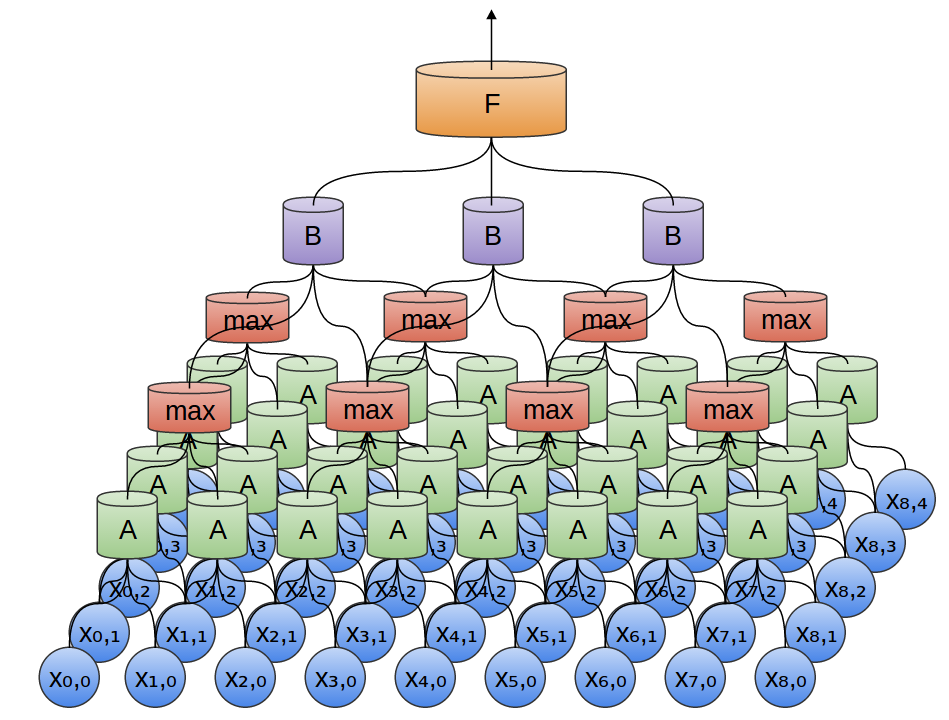
\includegraphics[width = 0.7\linewidth]{images/conv3.png}
\caption{Added max pooling to previous net}
\label{fig:principle}
\end{figure}

\end{frame}

\begin{frame}{Second Trick: Pooling}
  \begin{itemize}
  \item 'zooms' out
  \item small patch after pooling corresponds to much larger patch before it
   \item makes the network a little more invariant to location of features
    \end{itemize}
\begin{figure}
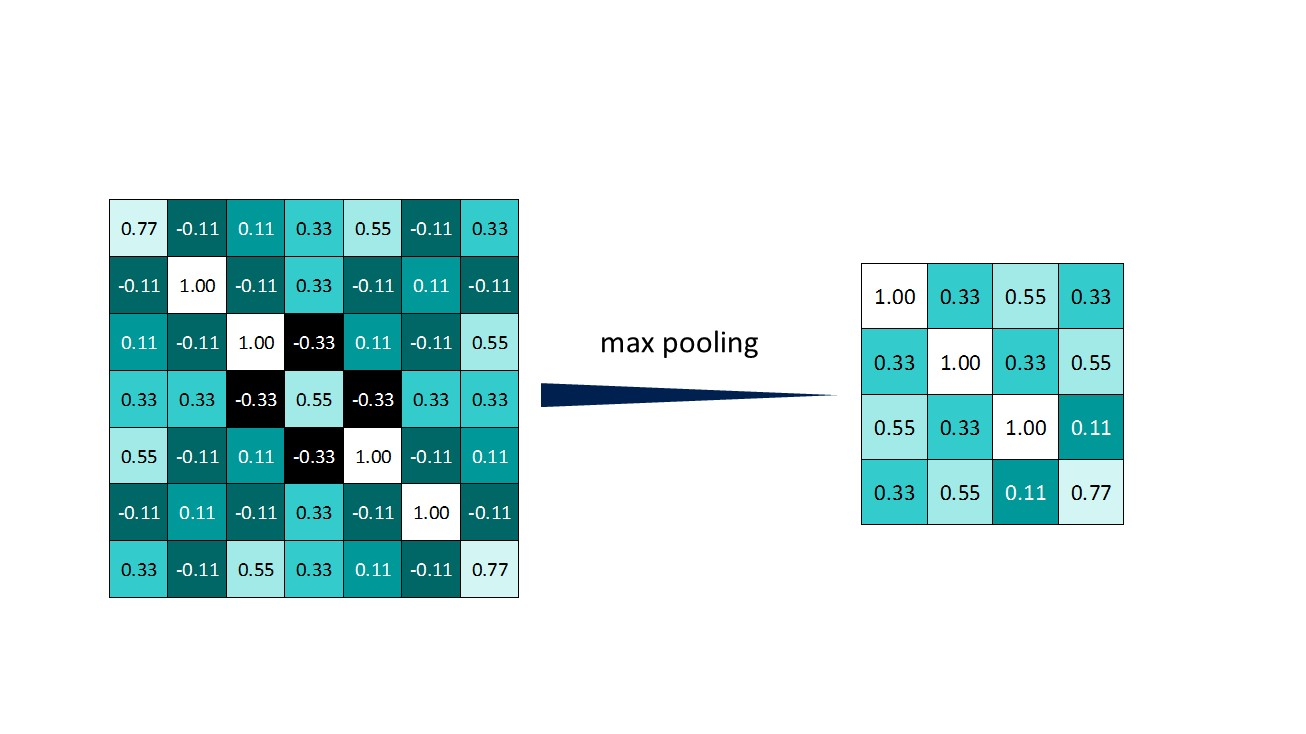
\includegraphics[width = 0.8\linewidth]{images/pooling.jpg}
\caption{Features}
\label{fig:principle}
\end{figure}

\end{frame}

\begin{frame}{Stacking Layers}
  \begin{itemize}
  \item layers are composable
   \item we can feed the output of one layer into the input of another
   \item with each layer, we can detect higher level, more abstract features
    \end{itemize}
\begin{figure}
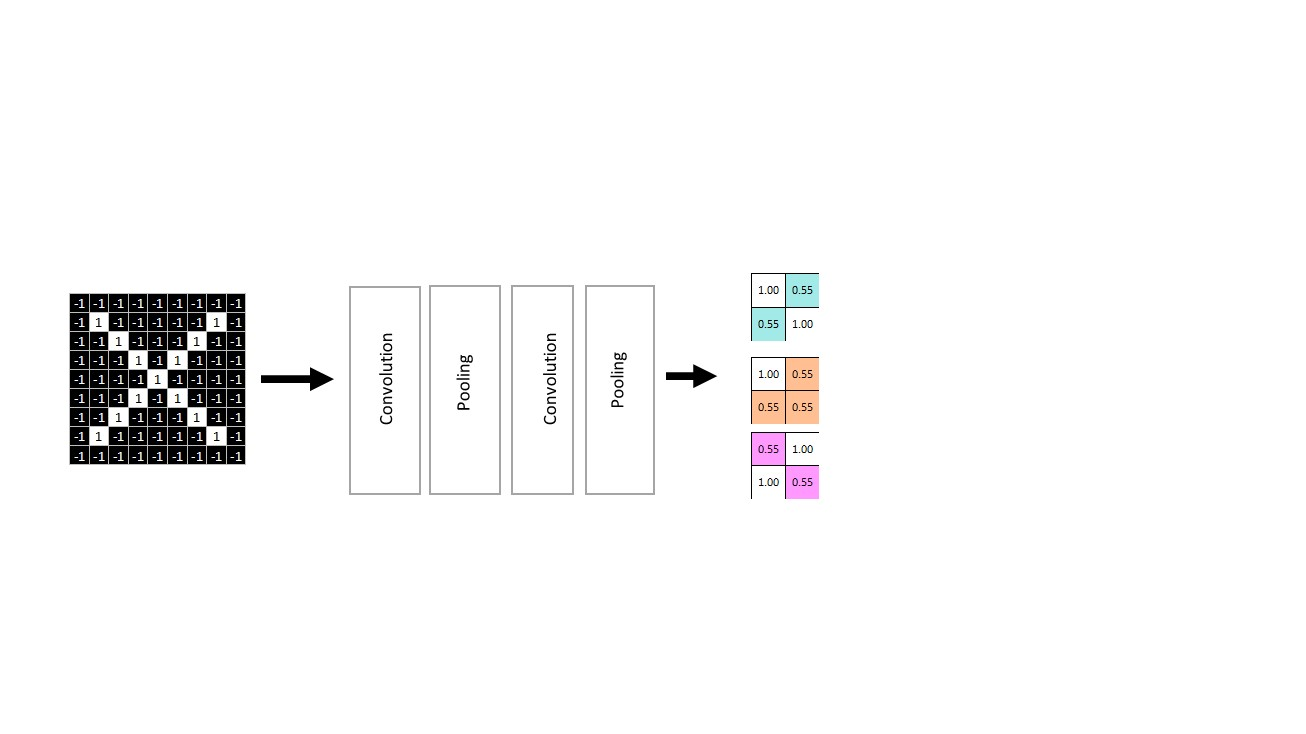
\includegraphics[width = 0.9\linewidth]{images/stacking.jpg}
\caption{Features}
\label{fig:principle}
\end{figure}

\end{frame}

\begin{frame}{Stacking Layers}
\begin{figure}
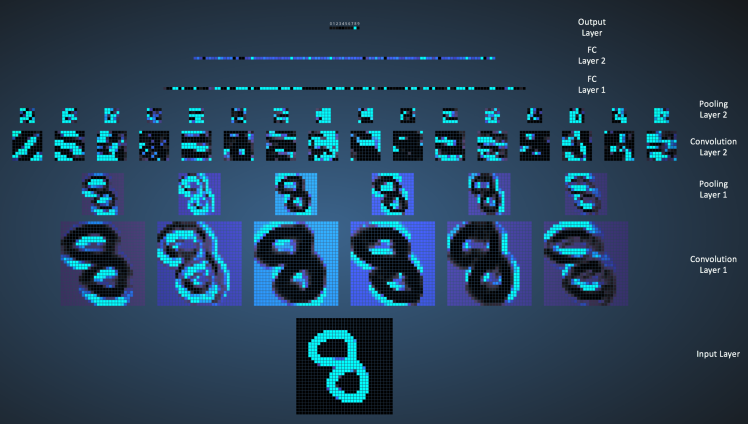
\includegraphics[width = 1\linewidth]{images/chain.png}
\caption{Visualizing a ConvNet trained on handwritten digits}
\label{fig:principle}
\end{figure}

\end{frame}

\begin{frame}{Structure}
\begin{figure}
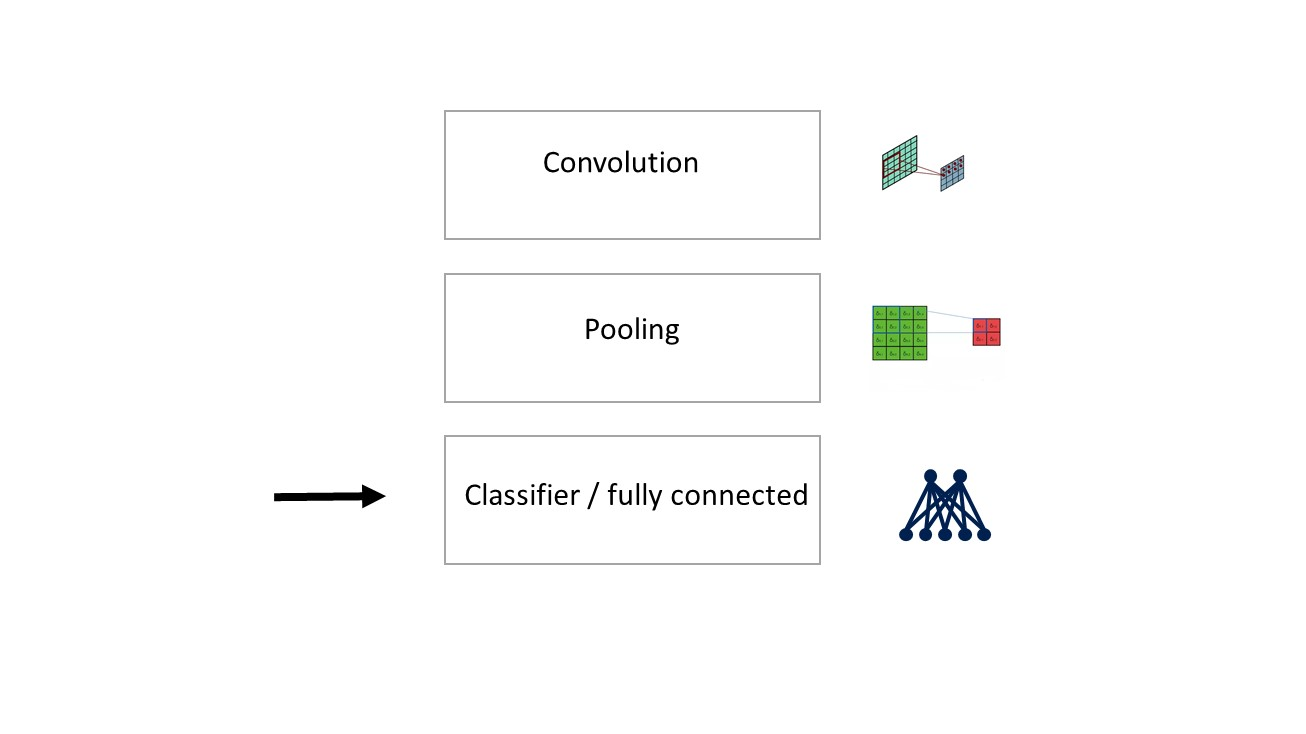
\includegraphics[width = 1\linewidth]{images/struct3.jpg}
\label{fig:principle}
\end{figure}
\end{frame}

\begin{frame}{Third Trick: Fully Connected}
  \begin{itemize}
  \item every value in a fully connected layer gets a 'vote' which affects the result of classification
  \item values in certain positions are associated with a certain class
    \end{itemize}
\begin{figure}
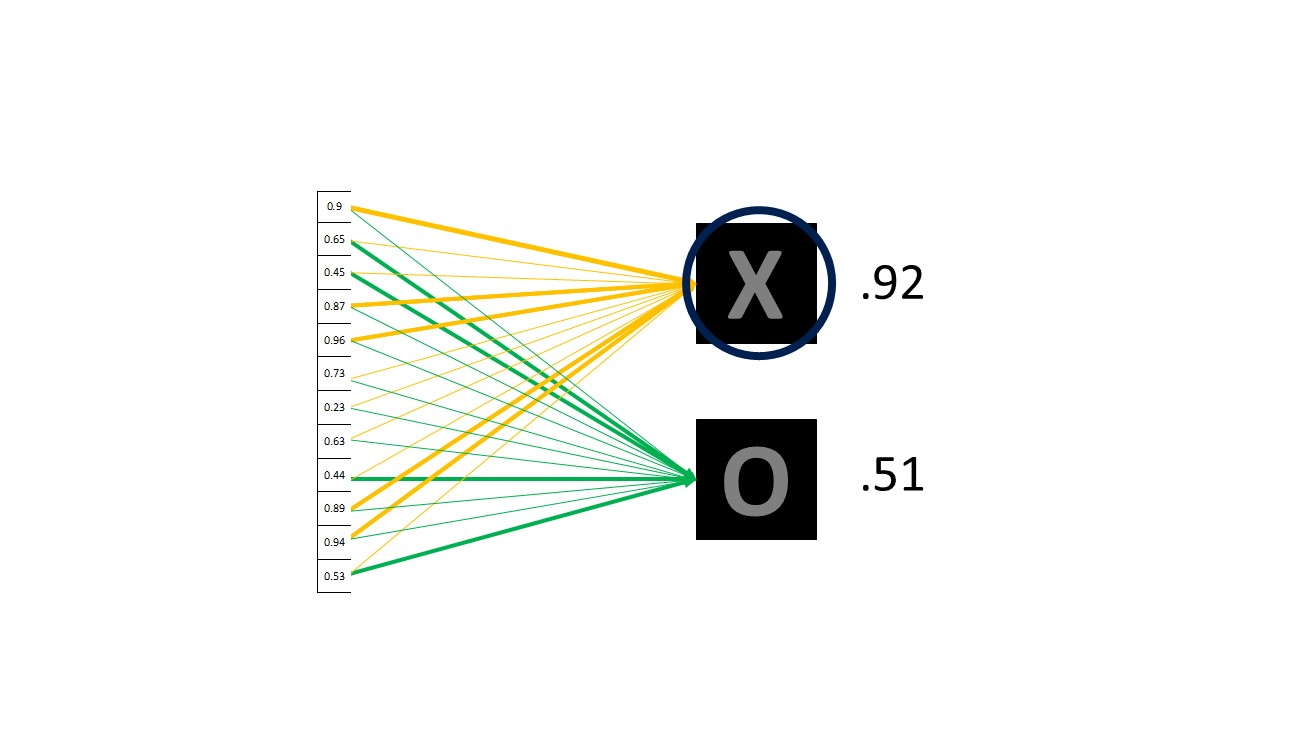
\includegraphics[width = 0.8\linewidth]{images/fc.jpg}
\caption{Weights in a fully connected layer contributing to classification}
\label{fig:principle}
\end{figure}

\end{frame}























\section{Components}
\begin{frame}{Our approach}
\centering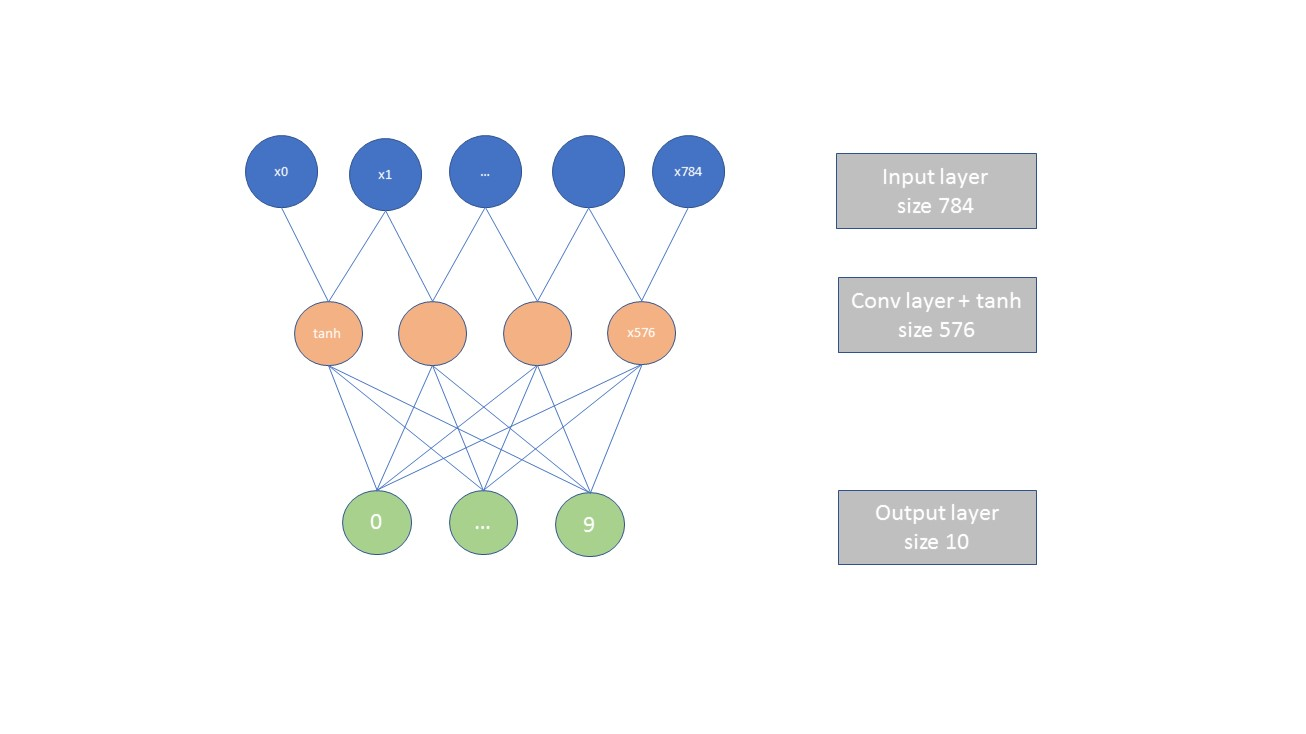
\includegraphics[width =1\linewidth]{images/ournet.jpg}



\end{frame}

\begin{frame}{Our approach - forward propagation}
\centering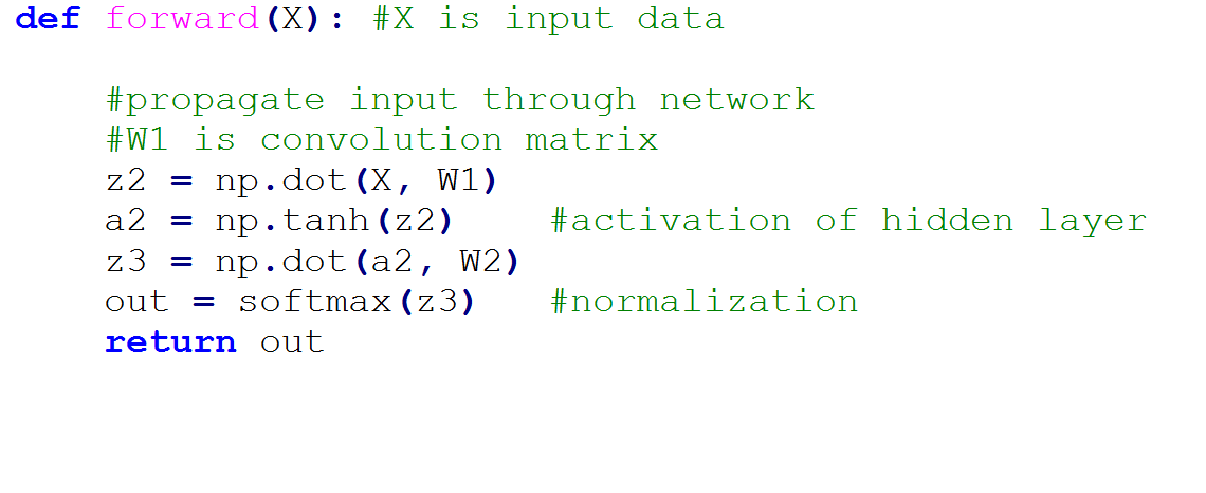
\includegraphics[width =1\linewidth]{images/forward.png}



\end{frame}
\subsection{Activation-function}
\begin{frame}{Activation function}
Activation-functions are typically used  to add nonlinearity to the network
\begin{figure}
\centering
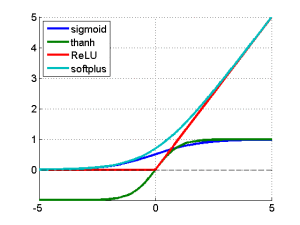
\includegraphics[width = 0.4\linewidth]{images/activation_functions.png}
\caption{Different activation-functions}
\label{fig:activation function}
\end{figure}
\begin{itemize}
\item activation functions must be non-linear and differentiable
\item the classification network uses the tangens-hyperbolicus function
\end{itemize}
\end{frame}




\subsection{Dense layer}

\begin{frame}{Fully connected layer}
The program's output layer is fully connected:
\begin{figure}
\centering
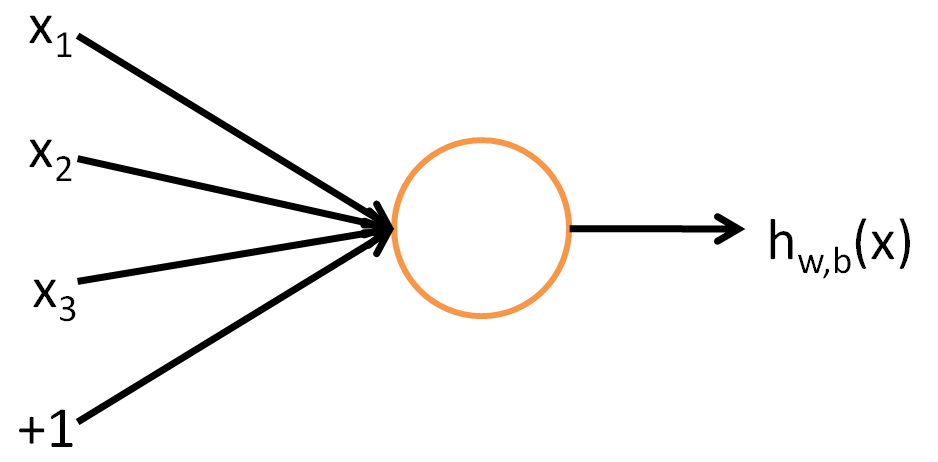
\includegraphics[width = 0.6\linewidth]{images/SingleNeuron.png}
\caption{Single neuron in a fully connected layer}
%todo: schöneres Bild
\label{fig:principle}
\end{figure}

Output:\space\space\space\space\space\space\space$(\sum_{i}{w_i x_i})$ \newline



\end{frame}


\subsection{Convolutional layer}

\begin{frame}{Convolutional layer}
Since iterating over the image each time is computationally inefficient, a mathematical representation is formed:\newline
%TODO
\centering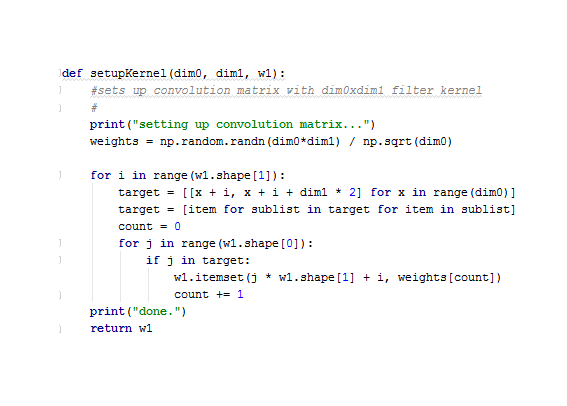
\includegraphics[width = 0.6\linewidth]{images/codekernel.png}
\begin{itemize}
\item Input: \space$conv = x*W_1 + b_1$ 
\item Output: $out = tanh(conv)$ 
\end{itemize}
\end{frame}



\subsection{Training}
\begin{frame}{Training}
\large
%todo: Bild von etwas mit backpropagation
The program was trained with backpropagation: \newline \newline
Backpropagation is the key algorithm which makes training neural networks feasible by greatly increasing the efficiency of learning algorithms.
\newline
To understand backpropagation, it is necessary to introduce the concept of forward propagation:

\end{frame}


\begin{frame}{Forward propagation}
Forward propagation is  the process of computing the output of a network for a given input:



\begin{figure}
\centering
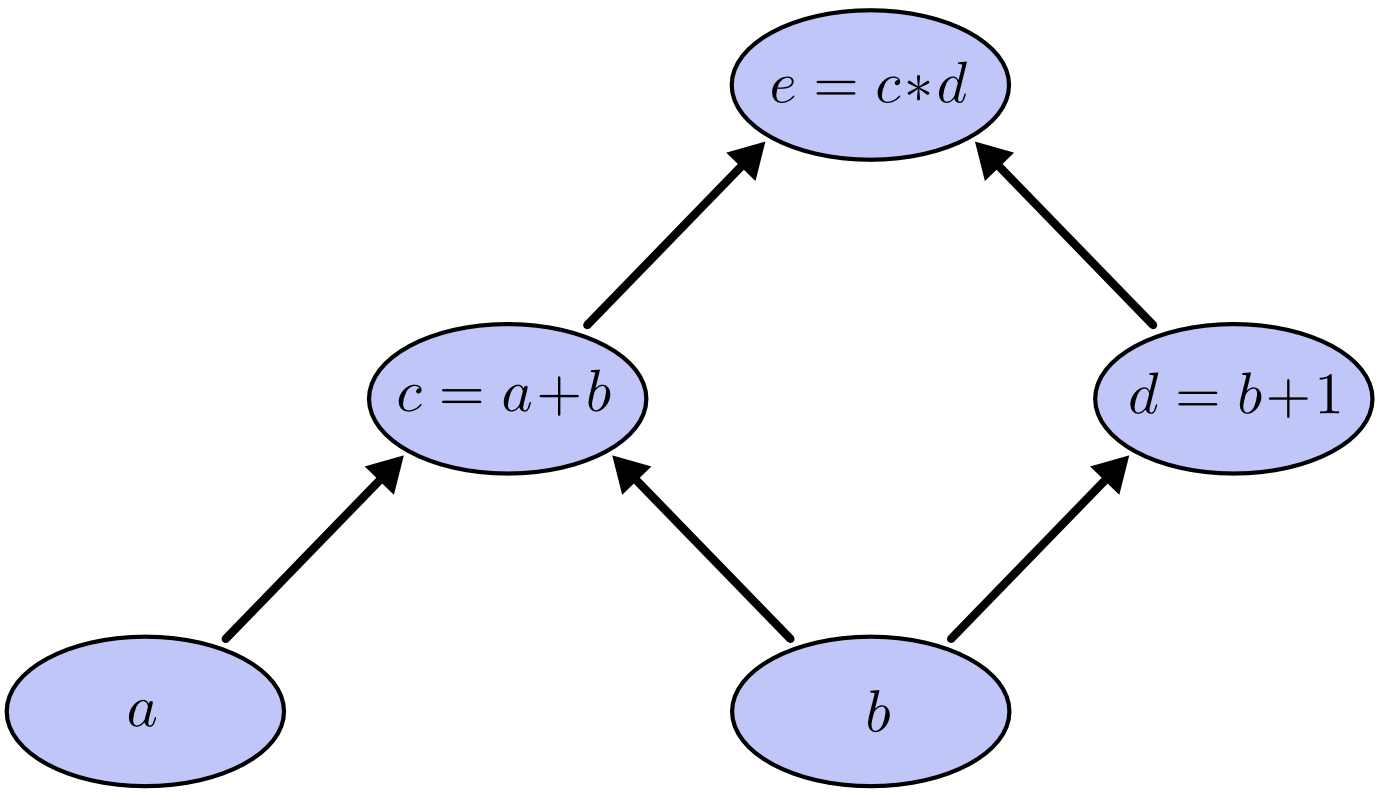
\includegraphics[width = 0.6\linewidth]{images/backprop1.png}
\caption{Computational graph of $e = (a+b)\cdot (b+1)$}

\label{fig:propagation}
\end{figure}
\end{frame}

\begin{frame}{Forward propagation}

The input is arbitrarily set to $a = 2$ and $b = 1$

\begin{figure}
\centering
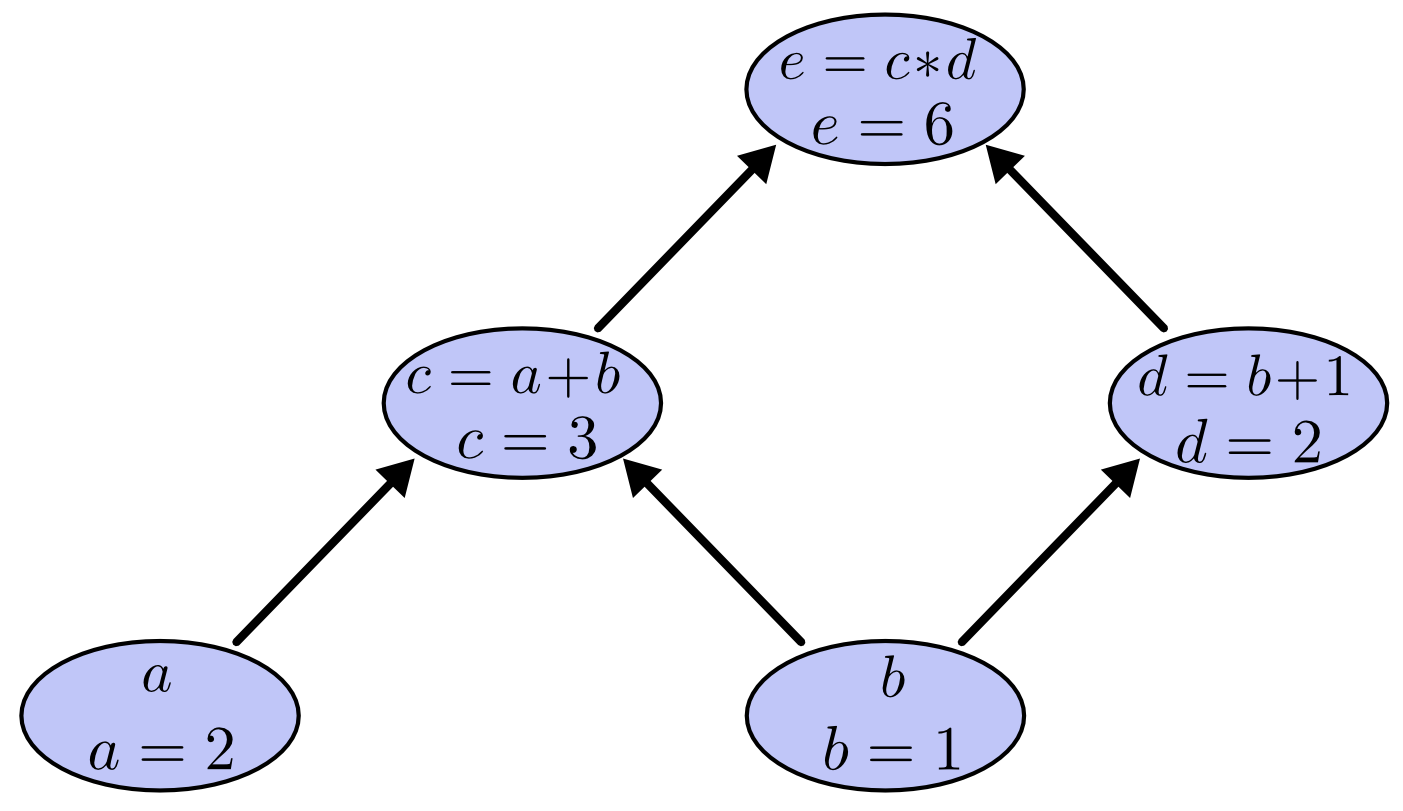
\includegraphics[width = 0.6\linewidth]{images/backprop2.png}
\caption{Computational graph of $e = (a+b)\cdot (b+1)$}

\label{fig:propagation}
\end{figure}
\end{frame}
\begin{frame}{Forward propagation}
\begin{itemize}
\item 
To train network weights one must determine how the output is influenced by its layer weights.
\item
This is achieved by finding the respective partial derivatives
\end{itemize}

\bigbreak

$c$ is only indirectly influenced by $a$ and $b$. To derive the exact influence, the chain rule can be applied:\newline

\large$\frac{\partial{e}}{\partial{a}} = \frac{\partial{e}}{\partial{c}} \cdot \frac{\partial{c}}{\partial{a}}$
\newline \newline
\large$\frac{\partial{e}}{\partial{b}} = \frac{\partial{e}}{\partial{d}} \cdot \frac{\partial{e}}{\partial{c}} \cdot \frac{\partial{d}}{\partial{b}} \cdot \frac{\partial{c}}{\partial{b}}$



\end{frame}
\begin{frame}{Forward propagation}
\begin{figure}
\centering
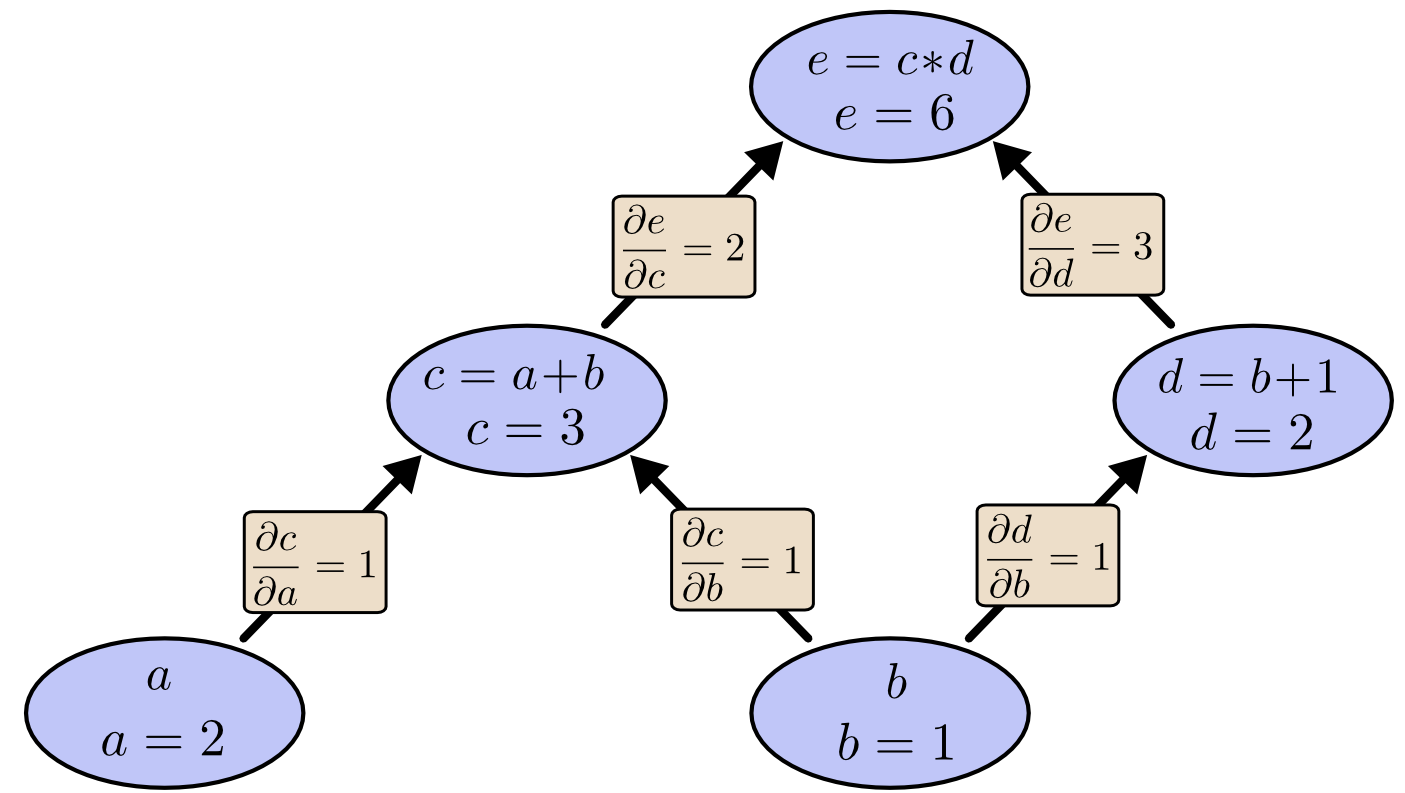
\includegraphics[width = 0.4\linewidth]{images/backprop3.png}

\label{fig:propagation}
\end{figure}
\begin{itemize}
\item This approach works for training networks
\item Problem: exponential number of derivatives might be necessary
\end{itemize}
\begin{figure}
\centering
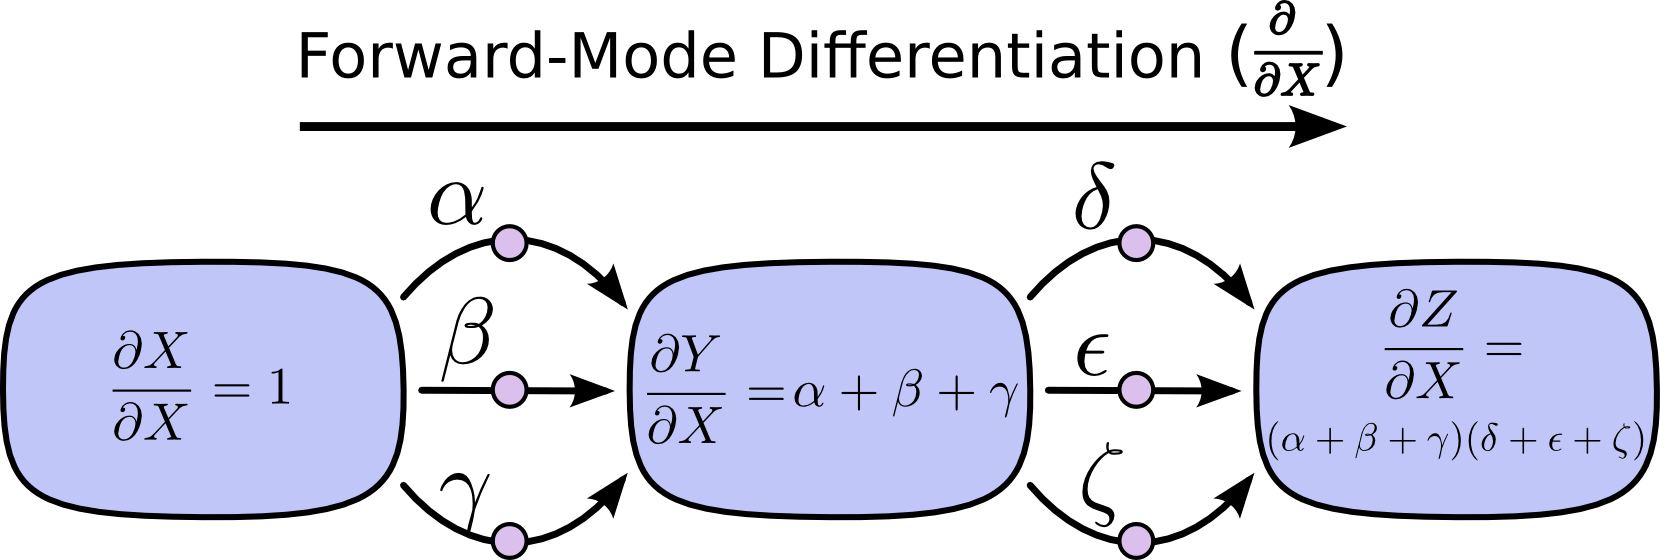
\includegraphics[width = 0.5\linewidth]{images/backprop5.png}
\label{fig:propagation5}
\end{figure}
\end{frame}

\begin{frame}{Solution: Backpropagation}
Instead of determining the influence of each input on the output, the influence of the layers on the output is influenced by the previous layers.

\begin{figure}
\centering
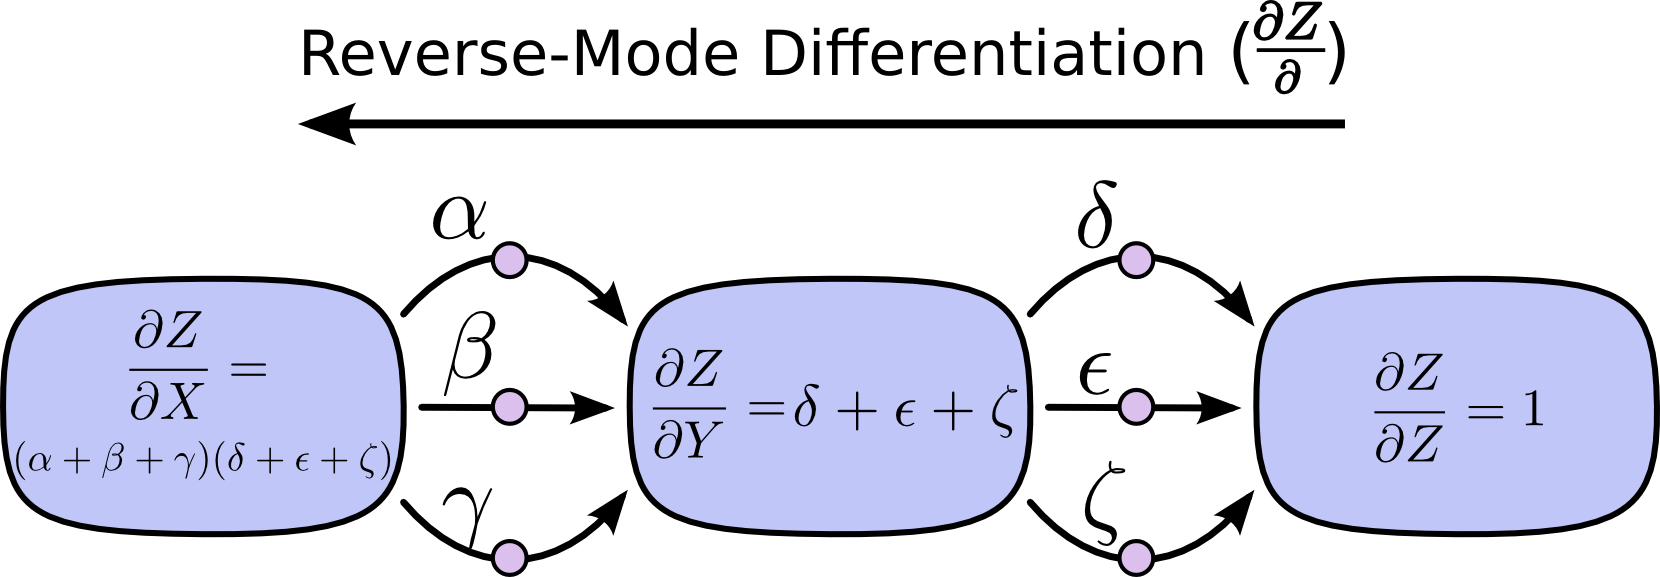
\includegraphics[width = 0.6\linewidth]{images/backprop6.png}
\label{fig:propagation5}
\end{figure}

\end{frame}

\begin{frame}{Backpropagation}
In the previous example executing a backward differentation immediately gives us the derivative of the output relative to every input:
 

\begin{figure}
\centering
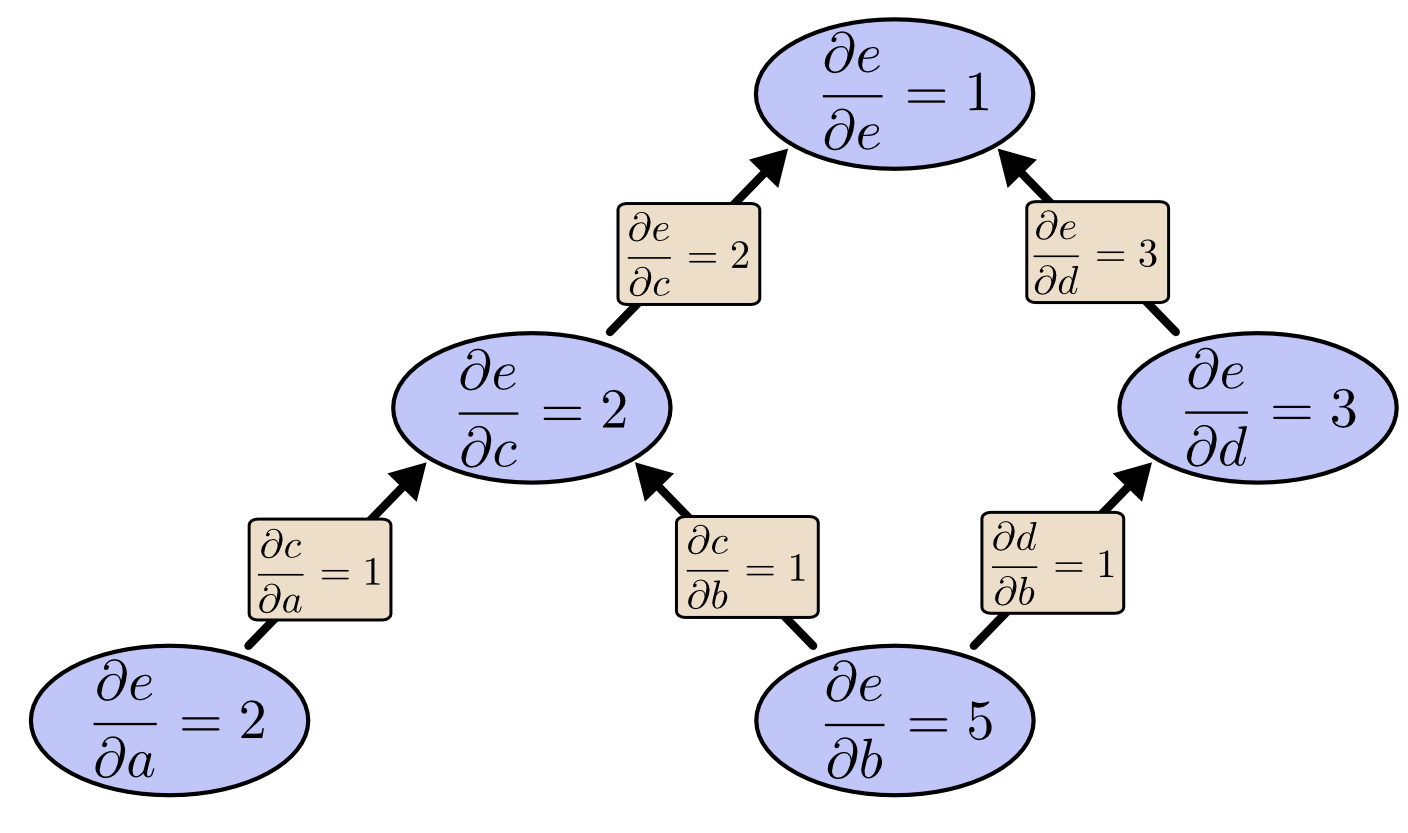
\includegraphics[width = 0.4\linewidth]{images/backprop7.png}
\label{fig:propagation5}
\end{figure}
This allows for massive speedup in networks with many inputs
\end{frame}



\begin{frame}{Backpropagation}
Math behind the classification program: \newline \newline

Convolution:\space\space\space\space\space\space\space\space\space\space\space\space\space\space\space\space\space\space                   $conv = x \cdot W_1 +b_1$ \newline
Convolutional layer output:\space\space\space\space    $out = tanh(conv)$\newline
Fully connected layer output:\space\space  $\hat{y} = out \cdot W_2 + b_2$\newline
Loss function:\space\space\space\space\space\space\space\space\space\space\space\space\space\space\space\space				   $L = - \sum_{N} y \cdot \ln{\hat{y}}$ \newline
\newline \newline
The training function will attempt to minimize the loss function in regards to the parameters. \newline
\end{frame}
\begin{frame}{Backpropagation}
The four trainable parameters in the program are:
\begin{enumerate}
\item$W_1$: weight of convolutional layer
\item$W_2$: weight of fully connected layer
\item$b_1$: offset of convolutional layer
\item$b_2$: offset of fully connected layer
\end{enumerate}

\end{frame}
\begin{frame}{$W_2$: Weight of fully connected layer}
\begin{Large}
$\frac{\partial{L}}{\partial{W_2}} = \frac{\partial{L}}{\partial{\hat{y}}} \cdot \frac{\partial{\hat{y}}}{\partial{W_2}}$
\newline  \newline
$\frac{\partial{L}}{\partial{\hat{y}}} = \sum_{N} y \cdot \frac{\partial{\ln{\hat{y}}}}{\partial{\hat{y}}} = \hat{y}-y$\newline
$\frac{\partial{\hat{y}}}{\partial{W_2}} = \frac{\partial{\hat{out \cdot W_2 +b_2 }}}{\partial{W_2}}= out^T$ \newline\noindent\makebox[\linewidth]{\rule{\paperwidth}{0.4pt}} \newline
\textbf{$ = (\hat{y} - y) * out^T $}
\end{Large}
\end{frame}




\begin{frame}{$b_1, b_2$: Offset of both layers}
\Large
$\frac{\partial{L}}{\partial{b_1}} = \frac{\partial{L}}{\partial{\hat{y}}} \cdot \frac{\partial{\hat{y}}}{\partial{out}}\cdot \frac{\partial{out}}{\partial{conv}} \cdot \frac{\partial{conv}}{\partial{b_1}} = $
\newline\noindent\makebox[\linewidth]{\rule{\paperwidth}{0.4pt}}
$ =  (1-tanh^2{conv}) \cdot (y-\hat{y}) \cdot W_2 \cdot 1$ \newline \newline
$\frac{\partial{L}}{\partial{b_2}} = \frac{\partial{L}}{\partial{\hat{y}}} \cdot \frac{\partial{\hat{y}}}{\partial{b_2}}$\newline\noindent\makebox[\linewidth]{\rule{\paperwidth}{0.4pt}}
$ = (\hat{y}-y) \cdot 1$\newline \newline

\end{frame}
\begin{frame}{$W_1$: Weight of convolutional layer}
\large
$\frac{\partial{L}}{\partial{W_1}} = \frac{\partial{L}}{\partial{\hat{y}}} \cdot \frac{\partial{\hat{y}}}{\partial{out}}\cdot \frac{\partial{out}}{\partial{conv}} \cdot \frac{\partial{conv}}{\partial{W_1}}$
\newline
$\frac{\partial{\hat{y}}}{\partial{out}} = \frac{\partial{\hat{out \cdot W_2 +b_2}}}{\partial{out}} =W_2$
$\frac{\partial{out}}{\partial{conv}} = \frac{\partial{ tanh(conv)}}{\partial{conv}} = 1 - \tanh^2{conv}$ 
$\frac{\partial{conv}}{\partial{W_1}} = x^T$
\newline\noindent\makebox[\linewidth]{\rule{\paperwidth}{0.4pt}}

$\frac{\partial{L}}{\partial{W_1}} = x^T \cdot (1-tanh^2{conv}) \cdot (y-\hat{y}) \cdot W_2 $








\end{frame}



\begin{frame}{Backpropagation in the program}

\begin{figure}
\centering
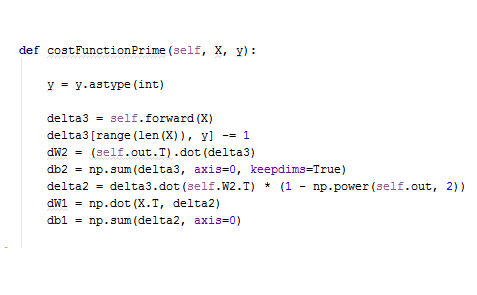
\includegraphics[width = 0.8\linewidth]{images/backpropagation.png}
\caption{Backpropagation in the program}
\label{fig:Backpropagation}
\end{figure}

\end{frame}

\section{Results}
\begin{frame}{Results}
\begin{figure}
\centering
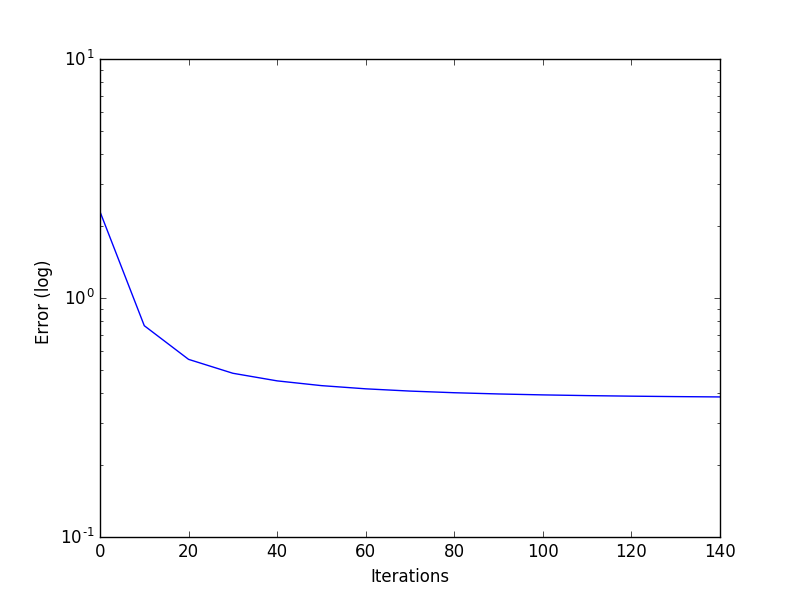
\includegraphics[width = 0.4\linewidth]{images/figure_1.png}
\caption{Training results}
\label{fig:principle}
\end{figure}
\begin{itemize}
\item The classification program was trained with 60000 images of digits from the MNIST database
\item Training results were tested by classifying 10000 other images
\item After training the program classifies images with an accuracy of approximately 92\%
\end{itemize}
\end{frame}
\begin{frame}{Results}
\begin{figure}
\centering
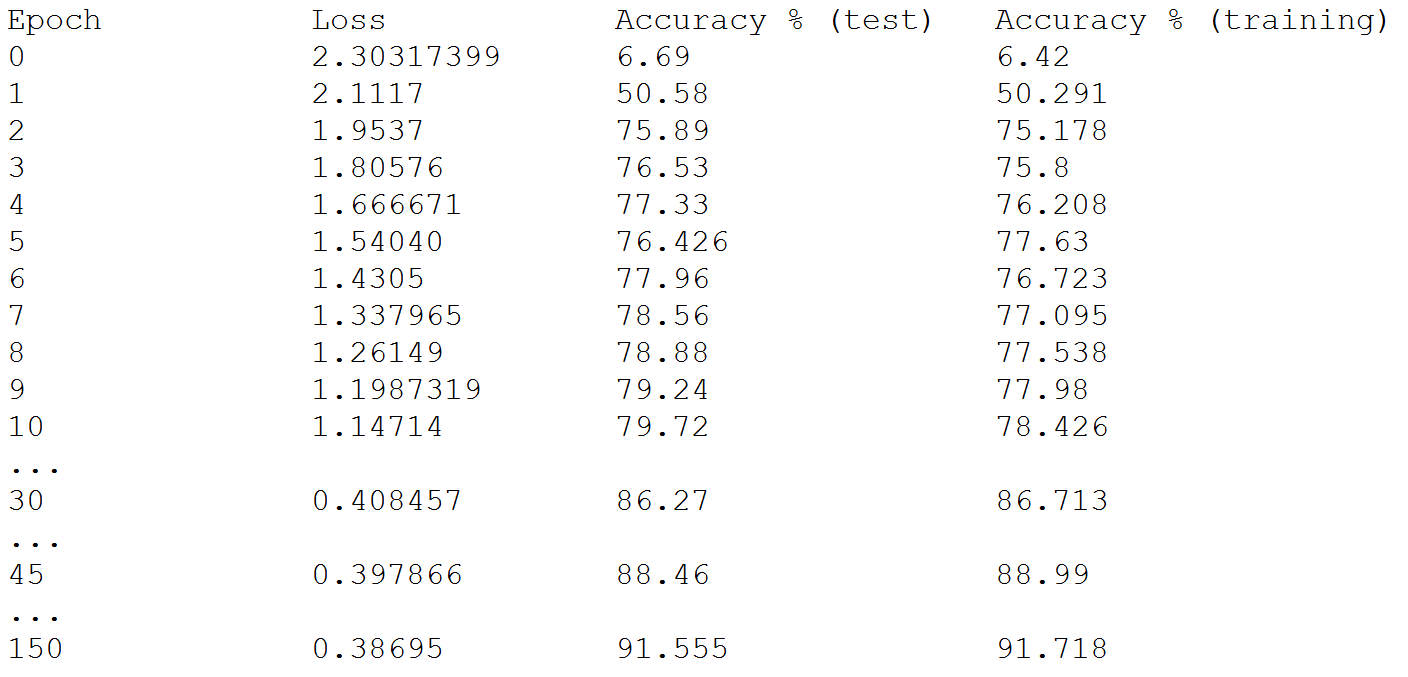
\includegraphics[width = 1\linewidth]{images/results.png}
\caption{Training results}
\label{fig:principle}
\end{figure}
\end{frame}
%todo: animal visual cortex
%\subsection{Layers}

%
%


\subsection{Application}
\begin{frame}{Application}
Visual Object Recognition
\begin{figure}
\centering
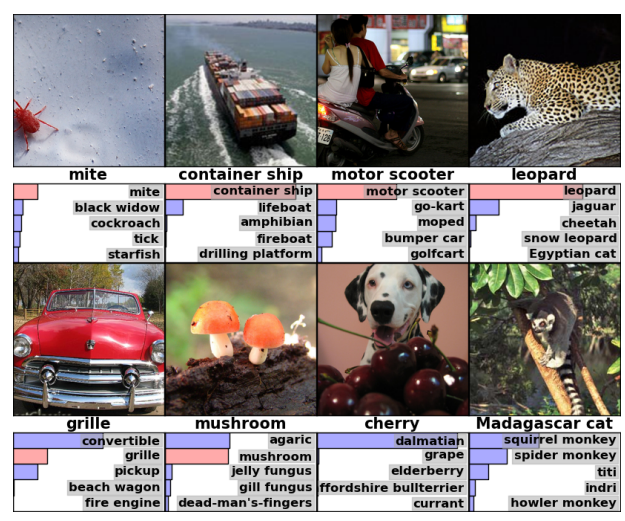
\includegraphics[width = 0.4\linewidth]{images/KSH-results.png}
\caption{ImageNet Classification with Deep Convolutional
Neural Networks}
\label{fig:principle}
\end{figure}
ImageNet by Krizhevsky et al (2012) classified 1.2 million
high-resolution images in the ImageNet LSVRC-2010 into 1000 different classes.
It achieves error rates of 37.5\% for the top result and 17.0\% for the top-5 results.


%The neural network, which has 60 million parameters and 650,000 neurons, consists
%of five convolutional layers, some of which are followed by max-pooling layers,
%and three fully-connected layers with a final 1000-way softmax

\end{frame}

\begin{frame}{Application}
Text Classification
\begin{figure}
\centering
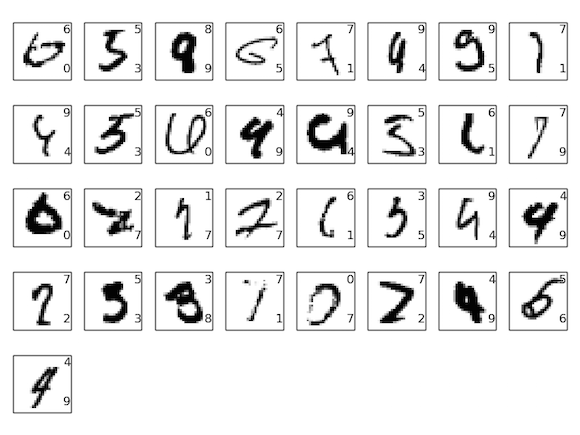
\includegraphics[width = 0.4\linewidth]{images/mnist.png}
\caption{Excerpt of MNIST}
\label{fig:principle}
\end{figure}
\end{frame}


\begin{frame}[fragile]
\footnotesize
\begin{verbatim}
http://blog.christianperone.com/2015/08/convolutional-neural-networks-and-feature-extraction-with-python/
http://cs231n.github.io/neural-networks-1/#bio
http://futurehumanevolution.com/artificial-intelligence-future-human-evolution/artificial-neural-networks
http://colah.github.io/posts/2014-07-Conv-Nets-Modular/
https://bfeba431-a-62cb3a1a-s-sites.googlegroups.com/site/deeplearningcvpr2014/ranzato_cvpr2014_DLtutorial.pdf?attachauth=ANoY7cpoT6OKao2g3iqQB4JqrLBF4e9GfZ06wOsnqfD_Dy5aob09rA3XzGPQSysUphYafHjkncEfoJPPyab19s4v8tfQS65Xk57NWieQOFC1zrYR2O_0gUN1Bsb64TS6kucrQP2prHjwwO4-Bc_9IRzGfWtlSMUGL_SxZnW_uSJHNbCzTQSfeZicjRxOCsBCNcA-4ifO2z8HaCqegyP8LQQGlp9gA7bPiIva1wxa69xKa7PB0iipEVWW180McZkDbBjefD0Thr13&attredirects=0
http://briandolhansky.com/blog/2013/9/27/artificial-neural-networks-backpropagation-part-4
http://neuralnetworksanddeeplearning.com/chap2.html
http://colah.github.io/posts/2014-07-Understanding-Convolutions/
http://neuralnetworksanddeeplearning.com/chap6.html
http://ufldl.stanford.edu/tutorial/supervised/MultiLayerNeuralNetworks/
https://imiloainf.wordpress.com/2013/11/06/rectifier-nonlinearities/
http://colah.github.io/posts/2014-07-Understanding-Convolutions/
https://colah.github.io/posts/2015-08-Backprop/
http://cs231n.github.io/convolutional-networks/
http://colah.github.io/posts/2014-07-Conv-Nets-Modular/
http://www.cs.toronto.edu/~fritz/absps/imagenet.pdf
\end{verbatim}
\end{frame}
\begin{frame}

\end{frame}
\begin{frame}
Additional Content which was overkill for the main presentation:
\end{frame}
\begin{frame} {Overfitting}

Overfitting occurs when the complexity of the model relative to the training size is too high.


The model begins memorizing the training data rather  than the underlying principle and easily loses its predictive power when the input is slightly altered.

Overfitting is prevented in a number of ways:

\begin{enumerate}

\item max-pooling layers
\item dropout layers
\item

\end{enumerate}

\end{frame}


\begin{frame}{Components - Neuron in convolutional layer}
To understand the concept behind Convolution we first demonstrate it in an example:
\begin{figure}
\centering
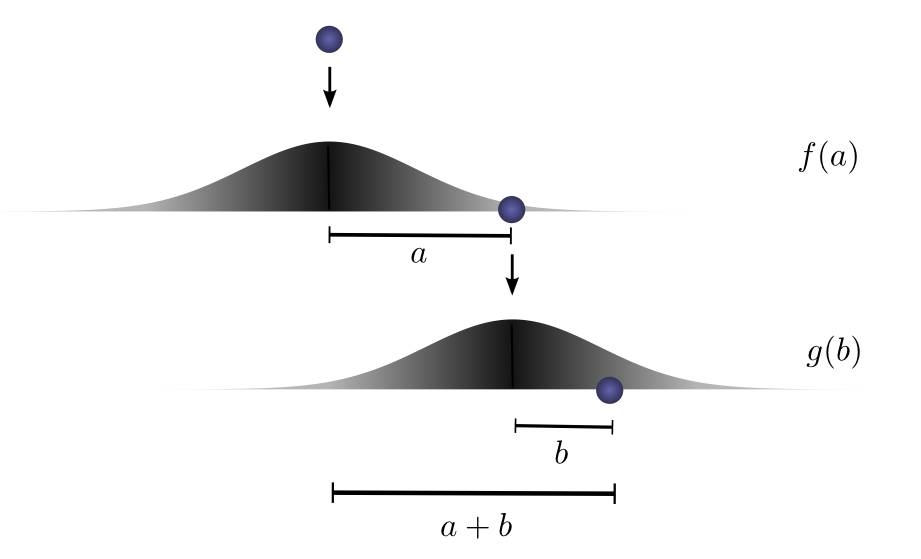
\includegraphics[width = 0.4\linewidth]{images/convprob.png}
\caption{Probability distribution of ball thrown twice}
\label{fig:principle}
\end{figure}
We want to calculate the likelihood of the ball traveling a distance $c$ after being thrown twice in a row. \newline


\end{frame}
\begin{frame}{Input}
\huge
Input layer
\newline
\normalsize
The input layer consists of an n-dimensional matrix, which contain the information to be processed

\begin{itemize}
\item Our example uses a 2-dimensional input which represents the pixels of the images
\item asd
\end{itemize}



\end{frame}


\begin{frame}
Input: \newline
$a, b$: length of first and second throw
$f(a), g(b)$: probability distribution of the balls location
If we want $c = a + b$ the probability of this event is $f(a) \cdot g(b)$

Since only the actual outcome is relevant to us, the actual values of $a$ and $b$ can be varied.

The total likelihood of the ball landing at $c$ can also be summed over all probability distributions where $a+b=c$:

$f*g(c) = \sum_{a+b=c} {f(a) \cdot g(a)} $

The result of this sum is a convolution between a and b
\end{frame}

\begin{frame}

\begin{figure}
\centering
Image processing with a kernel function can also be described as a convolution:
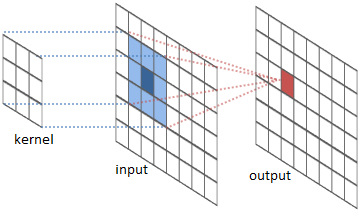
\includegraphics[width = 0.4\linewidth]{images/Kernelfunction.png}
\caption{Convolution between an input image and a kernel function}
\label{fig:principle}
\end{figure}

$out = \sum_{a} \sum_{b} w_{ab} \cdot x $



\end{frame}
\begin{frame}{Layers - Convolution}
The neurons of the Convolutional Layer is connected to the output of the previous layer through the kernel-function. 
\end{frame}

\begin{frame}{RELU/tanh layer}
%The RELU layer (from rectified linear units) is a fully connected layer which implements the threshold function $y  = max(0,x)$. It adds non linearity to the network, which would otherwise be identical to a single layer perceptron. This makes the approximation of nonlinear functions possible. \newline Recent research has found a different activation function, the rectified linear function, often works better in practice for deep neural networks. This activation function is different from sigmoid and tanh http://ufldl.stanford.edu/tutorial/supervised/MultiLayerNeuralNetworks/

because it is not bounded or continuously differentiable. The rectified linear activation function is given by,
f(z)=max(0,x).

To make backpropagation easier we used a differentiable function similar to RELU: $y = ln(1+e^x)$
\end{frame}

\begin{frame}{Max-Pooling layer}
The Max-Pooling layer partitions the image, returns the maximum value of each partition   and returns a compressed version of the input. This is done to a) reduce overfitting and b) downsampling the input


\end{frame}
\begin{frame}{Dropout Layer}
The dropout layer is a fully connected layer. It reduces overfitting and downsamples the input by randomly dropping neurons and their connections during training. 

\end{frame}
\begin{frame}{Dense layer}
The dense layer is identical to a normal neural network layer in that it is fully interconnected with every neuron of the previous layer.
\linebreak
image here
\end{frame}

\begin{frame}{Output layer}
The output layer is fully connected and unambigously assigns each neuron of the output to one of the expected results.
\linebreak
image here
\end{frame}
\end{document}